\documentclass[times, 10pt]{thesisMDH}
\addbibresource{references.bib}

% --- Pacages -----
\usepackage[ddmmyyyy]{datetime}
\usepackage{graphicx}
% \usepackage{epsfig} % Used to load plantuml
\usepackage{epstopdf} %converting to PDF
% \usepackage{amsmath} % Dep mathtools
\usepackage{amsfonts} % dep
\usepackage[utf8]{inputenc}
%% Maths
\usepackage{mathtools} % Loads asmath
\usepackage{fancyhdr}
\usepackage{enumerate}
\usepackage{pdflscape}
% \usepackage{listings}     % Do not list codes in paper use bellow.
% \usepackage{algpseudocode} % Algorithms instead of listings
\usepackage[noend]{algpseudocode}
%\usepackage{algorithm,algorithmic}
\usepackage{algorithm}
\usepackage{ragged2e}
% \usepackage[linesnumbered,vlined,ruled,scleft]{algorithm2e}
% \usepackage[titletoc]{appendix}

\usepackage[margin=3cm]{geometry}
\usepackage[absolute]{textpos}
\usepackage[section]{placeins}
\usepackage{url}
\usepackage{tabularx}
\usepackage{acronym}
\usepackage{harpoon}  % Long vector arrows. perhaps DEP
\usepackage{gensymb}
\usepackage{caption}
\usepackage{subcaption}
\usepackage{todonotes}
\usepackage{multirow}
\usepackage{titlesec}

\usepackage{cprotect} % Use verb in figure captions

% Bibliography settings:

% \titleformat{\subsection}
% {\normalfont\small% Changed!
%   \bfseries}{\thesection}{1em}{}[{\titlerule[0.8pt]}]

\graphicspath{{Figures/}{figures/}{.}{images/}{results/}} %Setting the graphicspath

%%%%%%% Import tikz for a figure.
\usepackage{tikz}
% \usepackage{plantuml}
\usepackage{ifluatex}
\ifluatex
  \usepackage{pdftexcmds}
  \makeatletter
  \let\pdfstrcmp\pdf@strcmp
  \let\pdffilemoddate\pdf@filemoddate
  \makeatother
  \fi
\usepackage[clean]{svg}
% \usepackage{svg}
\svgpath{figures}

\usetikzlibrary{automata, positioning, arrows}
\tikzset{
    ->, % makes the edges directed
    >=stealth,
    %>=stealth’, % makes the arrow heads bold
    node distance=3cm, % specifies the minimum distance between two nodes. Change if necessary.
    every state/.style={thick, fill=gray!10}, % sets the properties for each ’state’ node
    initial text=$ $, % sets the text that appears on the start arrow
}
\tikzset{aruco/.style={
        rectangle, draw=black!50, fill=black!20, thick, minimum width=0.85cm, minimum height = 0.85cm,
    }
}
%%%%%%%% ----------------
%% =========={ Commando creation }==========
% \renewcommand\thesection{\arabic{section}}
% \newcommand{\lit}[1]{\item[\textbf{L#1}]
%\newcommand\req[1]{%
%    \item["\textbf{RQ#1}"]%
%    }%
% \newcommand\req[1]{\item[\textbf{RQ#1}]}
% \newcommand{\rew}[1]{{\color{red}#1}
% \newcommand{\rewc}[2]{{\color{#2}#1}
%\newcommand{\rewdetail}[2]{{\color{red}#1\todo[color=red!40]{#2}}
%\newcommand{\insertref}[1]{\todo[color=green!40]{#1}
%%\newcommand{\explainindetail}[1]{\todo[color=red!40]{#1}}
%\newcommand{\setseparation}{\setlength\itemsep{0mm}
%\def\checkmark{\tikz\fill[scale=0.6](0,.35) -- (.25,0) -- (1,.7) -- (.25,.15) -- cycle;}
%\newcommand{\cspace}{\ensuremath{\mathcal{C}}


% \renewcommand{\headrulewidth}{0.4pt}
% \renewcommand{\footrulewidth}{0.4pt}
% \newcommand\node[2]{%
% \item[%
% \textbf{#1}%
% ] \textbf{#2}%
% }

% % \newcommand{\R}{\(\mathbb{R}\)}
\newcommand*\aruco[1]{ArUco#1}
\newcommand*\openpose[1]{OpenPose#1}
\newcommand*\Q[1]{$Q_#1$}
\newcommand*\R{\mathbb{R}}
\newcommand*\defref[1]{Definition~\ref{#1}}
% \newcommand*\NN{\mathbb{N}} % natural numbers
\newcommand*\NN{\mathbb{N}} % natural numbers
\newcommand*\AAA{\mathcal{A}} % automaton
\newcommand*\WWW{\mathring{W}^2_1} % Sobolev space 2,1,o
\newcommand*\defined[1]{\emph{#1}} % used for defining new terms
\DeclarePairedDelimiter\abs{\lvert}{\rvert} % proper absolute value

% Larger \mu and \sigma for hypothesis question
\newcommand{\bigmu}{\makebox{\Large\ensuremath{\mu}}}
\newcommand{\bigsigma}{\makebox{\Large\ensuremath{\sigma}}}
% \newcommand{\bigmu}{\raisebox{-.20\baselineskip}{\ensuremath{\mu}}}
% \newcommand{\bigsigma}{\raisebox{-.20\baselineskip}{\ensuremath{\sigma}}}

\newcommand{\annoterel}[2]{%
  \overset{%
    \substack{\hidewidth\text{#1}\hidewidth\\\downarrow}%
  }{#2}%
}


\usepackage[pdfborder={0 0 0},colorlinks=true,urlcolor=blue,citecolor=red,bookmarks=false]{hyperref}


%%%%% Title page settings
\fancyHeader{Valid OpenPose on laying humans}{Magnus Sörensen}
\university{Mälardalen University}
\department{School of Innovation Design and Engineering\\ Västerås, Sweden}
\subject{Thesis for the Degree of Master of Science in Engineering - Robotics 30.0 credits}
\thesisTitle{Validation of OpenPose on laying humans using statistics, Aruco corners and a novel minimal point of error}
\authorOne{Magnus Sörensen}{msn15018@student.mdh.se}
%\authorTwo{Student Name2}{studentEmail@student.mdh.se}


\examiner{Martin Ekstr\"{o}m}{M\"{o}lardalen University, V\"{ä}sterås, Sweden}
\supervisorA{Fredrik Ekstrand}{M\"{a}lardalen University, V\"{a}sterås, Sweden}
\supervisorB{Joaqu in Ballestero}
{University of M\'{a}laga, M\'{a}laga, Spain}
\supervisorC{Jesus Manuel Gomez de Gabriel Ballesteros}{University of M\'{a}laga, M\'{a}laga, Spain}

\theDate{\today}
%%%%% END

\begin{document}
\titlePage
% Begin actual text
\frontmatter
%\section*{Introduktion: om begrepp som används i mallen}

I mallen använder vi ett antal begrepp som det är viktigt att ha klart för sig vad de avser och hur de relaterar till varandra.
Vi illustrerar detta med exempel.
Du kan ha fått ditt examensarbete som ett uppdrag från t ex ett företag.
I så fall har du ofta fått ett problem som företaget upplever och som du ska försöka hitta lösning på. 
Problemet utgör i detta fall bakgrunden till syftet med arbetet och den frågeställning som du arbetar fram.

Exempel: Företaget X har ett system som de vill kunna använda i en realtidstillämpning, men prestanda i systemet är okänt. 
Problemet är då: Prestanda i systemet är okänt.
Lösningen på problemet är att mäta prestanda.
Syftet med ditt arbete blir att kartlägga systemets prestanda så att du får ett mått på detta. 
Frågeställningen kan formuleras som: Vad är systemets prestanda? Motivationen för arbetet är att det är viktigt att känna prestanda när systemet ska användas för realtidstillämpningar.
När du har syfte och frågeställning klar formulerar du de mål som du ska uppfylla med arbetet, i det här fallet kan målen t ex vara att mäta ett antal olika aspekter av prestanda. 
Tillsammans kommer dessa mål då att uppfylla syftet. 
Men ditt examensarbete behöver inte vara formulerat som ett specifikt problem som ska lösas.
Andra exempel på arbeten som kan förekomma som examensarbeten kan vara:
\begin{itemize}
\item[--]	``Case study'' eller studie av något fenomen
\item[--]	Litteraturstudie
\item[--]	Undersöka något, t ex hur användare interagerar med en mjukvara eller hur en design kan anpassas till en viss grupp användare
\item[--]	Analysera t ex jämföra prestanda hos olika programvaror
\item[--]	Utvärdera hänger ofta ihop med att analysera något, din uppgift kan vara att lämna en rekommendation om vilket verktyg som bäst lämpar sig för en viss uppgift
\item[--]	Utforska ny teknik eller nya angreppssätt. I detta kan ingå att utveckla en artefakt, t ex en mjukvara eller ett system. 
\item[--]	Utreda en frågeställning, t ex genom att göra en förstudie
\item[--]	Utveckla och utvärdera en algoritm, t ex för ett beräkningsproblem
\end{itemize}
Naturligtvis kan ditt examensarbete också innehålla flera av ovanstående komponenter. 
Gemensamt för alla examensarbeten är att de ska vara grundligt vetenskapligt förankrade, ett examensarbete får t ex inte vara enbart en implementation.

I många av exemplen ovan finns det inte något tydligt specificerat problem som ska lösas. 
Det kan istället röra sig om en fråga som du söker svar på, som i exemplet med utvärdering.
Men alla examensarbeten ska ha syfte, frågeställning och motivation. 
Frågeställningen ska vara utformad så att den går att besvara på något sätt genom det arbete du gör.
Men svaret kan vara abstrakt, det kan t ex vara att bidra till kunskap om frågeställningen.
I exemplet där uppgiften är att utforska en teknik, så skulle frågeställningen kunna vara ”Vilka problem finns med att utveckla XX”?
Det är också vanligt att arbetet innebär att du ska analysera och/eller utvärdera artefakten du utvecklat.
Frågeställning och syfte ska matcha varandra på så sätt att när syftet är uppnått så besvaras frågeställningen.
I texten kommer vi att använda begreppet uppgift för det du ska göra, vare sig det är ett problem som ska lösas eller något annat.
Texten i mallen är i denna version på svenska, men för varje rubrik finns motsvarande engelska ord inom parentes.

Denna sida ska inte ingå i slutrapporten
\newpage % Remove 000-guideline section
% ============================= Abstract ==============================
\begin{abstract}
% Det här avsnittet ska helt enkelt vara just detta: en sammanfattning av hela rapporten. En lämplig omfattning är c:a 200 – 250 ord.  En bra tumregel är att sammanfattningen ska hållas så kort det går, den ska vara kompakt men fortfarande tydlig, informativ och väcka intresse. Ge de viktigaste fakta
% och summera allt det som är väsentligt i rapporten.  Följande bör ingå:
% \begin{itemize}
% \item[--]	Presentation/introduktion av området för arbetet
% \item[--]	översiktlig presentation av uppgiften inklusive syfte och frågeställning
% \item[--]	Motivation till varför området och uppgiften är viktiga och intressanta
% \item[--]	Generell beskrivning av hur du angripit uppgiften, vad du har gjort
% \item[--]	Sammanfattning av resultat och slutsatser och vad ditt arbete bidrar med
% \end{itemize}

% Inga detaljer ska vara med i sammanfattningen, inte heller beskrivning av hur rapporten är uppställd.
% Sammanfattningen ska kunna läsas helt fristående från resten av rapporten, och av en ganska bred grupp av läsare. Den ska ge en bra grund för att en läsare ska kunna bedöma om hen är intresserad av att läsa hela rapporten.
% Sammanfattningen är den del av en rapport som läses allra mest och av flest personer. Därför är det extra viktigt att du skriver en bra sammanfattning. Du behöver ha ett ordentligt grepp om innehållet i rapporten när du skriver sammanfattningen, och när hela rapporten är klar bör du granska och vid behov revidera sammanfattningen så att den överensstämmer med rapporten.
    \todo[inline]{Missing right now, comming later.}
\end{abstract}
\newpage
%%========= Tables ==========
{\hypersetup{linkcolor=black}\tableofcontents}
\clearpage
{\hypersetup{linkcolor=black}\listoffigures}
\clearpage
{\hypersetup{linkcolor=black}\listoftables}

\mainmatter
\section*{Acronyms}
\begin{acronym}[MPC] % Give the longest label here so that the list is nicely aligned
    %\acro{MPC}{model predictive control}
    %\acro{ros}[ROS]{Robot Operating System}
    %\acro{2d}[2D]{two-dimensional}
  %  \acro{3d}[3D]{three-dimensional}
    %\acro{dof}[DOF]{Degrees Of Freedom}
    \acro{uma}[UMA]{University of Malaga}
    \acro{mdh}[MDH]{University of Märlardalen}
    %\acro{ompl}[OMPL]{Open Motion Planning Library}
    %\acro{stomp}[STOMP]{Stochastic Trajectory Optimization for Motion Planning}
    %\acro{rrt}[RRT]{Rapidly exploring Random Tree}
    %\acro{t-rrt}[T-RRT]{Transitionbased Rapidly exploring Random Tree}
    %\acro{cnn}[CNN]{Convolutional Neural Network}
    %\acro{gnn}[GNN]{Generative Neural Network}
    %\acro{rpm}[RPM]{Relative Position Map}  % <- fix this one
    %\acro{spars}[SPARS]{SPArse Roadmap Spanners}
    %\acro{hri}[HRI]{Human Robot Interaction}
    %\acro{phri}[pHRI]{Physical Human Robot Interaction}
    % \acro{cum}[CUM]{Camera Utility Mechanism}
    %\acro{cum}[RCPA]{Radial Camera Position Armature}
    %\acro{}[RPi]{Raspberry Pi}
    \acro{ar}[AR]{Augmented Reality}
    \acro{slp}[SLP]{Simultaneously-collected multimodal Lying Pose}
    \acro{rgb}[RGB]{RGB color space}
    \acro{rgbd}[RGBD]{RGB color space with depth}
    \acro{lwir}[LWIR]{Long-wave infrared}
    \acro{slam}[SLAM]{Simultaneous Localization and Mapping}
    \acro{vslam}[VSLAM]{Visual Simultaneous Localization and Mapping}
    \acro{vr}[VR]{Virtual reality}
    \acro{sfm}[SfM]{Structure from Motion}
    % \acro{}[]{}
    % \acro{}[]{}
    % \acro{}[]{}
    % \acro{}[]{}
    % \acro{}[]{}
    % \acro{}[]{}
    % \acro{}[]{}
    % \acro{}[]{}
\end{acronym}

\newpage
% ===== Content: Modify the structure according to your needs =======
\section{Introduction}%
\label{sec:intro}
At \ac{uma} there is a robot intended to be used in helping the elderly if they have fallen on the floor.
In their approach, they are set on using \openpose to find and assist the elderly.
Thus it is relevant to investigate how \openpose reacts if an elderly human is lying on the ground.
% robot is used to either assist or pick them up.
%In this thesis, an investigation to how OpenPose
The problem is that OpenPose only seems to be trained on datasets where humans are standing, sitting, walking and running.
The missing data will be attempted to be solved using an inside out approach using a regular camera and ArUco conner take an image set.
Several images were taken around the subject on the ground and with at least one known ArUco corner in the picture.
In this way, the camera pose is known for each picture; consequently, that can triangulate a feature in each image.
Features in this paper are a set of points of interest on a human body, primarily joints, eyes, nose, and belly.
The 2D annotation is done by both \openpose in~\cite{qiao2017openpose} and a human operator returning a list of each feature.
The benefit of that is that the bias in the \openpose  algorithm for humans in a particular orientation can be discovered.
The resulting data is a point cloud of each feature, formed by a median point algorithm explained in~\ref{sec:background}
By investigating the divination and mean from different cameras, there is also a possibility of identifying a spread if the subject is in different orientations.

The methods used in this paper attempt to compare the output data from how \opnepose with a human in the image domain of the dataset and 3D reconstruction for how \onpepose would react to a human laying on the floor in the global domain.
The image domain data is compared using F-test and T-test against a human sample.
While the 3D reconstruction uses \aruco and Dijkstra's to algorithm solve the 3D position of the camera without solving the Bundle Adjustment problem.
% Later, that was proven to be unsolvable due to a cumulative error when traversing the nodes.

\subsection{Structure of this report}%
\label{sub:Structure_of_this_report}

The general structure of this document is as follows:
Section~\ref{sec:background} contains the initial thorough and general introduction to some of the subjects and math in this paper.
After the initial concept, the Related Works in\ref{sec:related_work} will discuss what others have done in this field of study.
Method\ref{sec:method} derives the necessary steps and forms a hypothesis to solve the problem.
There is an ethics section\ref{sec:ethics} that discusses the ethical part of this report.
The implementation section\ref{sec:work} discusses how it was implemented.
Results in section\ref{sec:results} show what the results were for the implementation.
Discussion\ref{sec:discussion} is the authors reflection on the results.
Conclusion\ref{sec:conclusion} summarizes the findings.
Appendices\ref{sec:appendices} contains tables and images used in this report.


% The resulting data is a point cloud of each feature, formed by a median point algorithm explained in~\ref{sec:background}
% \label{sec:s3d:ntroduction}
% \section{Results}\label{sec:results}
% \label{sec:method}
% \label{sec:background}
%\label{sec:bg}
% \label{sec:s3d:Method}




% \par The expected outcome from this project presented in point in~\ref{sub:expected_outocem} show what kind of data will be acquired and how that is supposed to be stored.




% \subsection{Hypothesis and research questions}%
% \label{sub:Hypothesis}
% The hypothesis for this job is that \openpose can not correctly identify the features of humans lying on the floor from certain angles.
% Thus, the hypothesis for this part of the work is:
% \vspace{5mm}
% \begin{itemize}
%     \item[$\mathbf{H_0}$] The standard deviation of \openpose is on pair with a human from all angles.
%     \item[$\mathbf{H_a}$] The standard deviation of \openpose significantly deviates at certain angles.
% \end{itemize}

% \vspace{5mm}
% \raggedright Research questions used to prove the hypothesis above.
% \begin{itemize}
%     \item[$\mathbf{Q_{1}}$] How does the accuracy of \openpose change as the camera is moving to a position where the subject is upside down?
%     \item[$\mathbf{Q_2}$] How does \aruco handle multiple fiducial markers in one image?
%     % \item[$\mathbf{Q_3}$]
% \end{itemize}

% \def\svgwidth{\columnwidth}
% \begin{figure}[ht]
%     \centering
%         % \input{Figures/validation.pdf_tex}
%         % \input{Figures/validation.pdf_tex}
%         \input{images/dataset.pdf_tex}
%       \caption{
%                       In this figure, the subject is on its back facing upward and from the for angles in the figure the two features marked as $F_{sr}$, $F_{er}$ for right shoulder and elbow respectively.
%           In the last image, its proposed the elbow can not be found from that camera angle thus not marked.
%           The \arucos  corner at the head is the origin for the system with corner 0.
%           Also for the last image, the camera cannot observe the origin, but as each other \arucos  corners is observed from the other angle, the camera position can still be calculated from the other \arucos  corners.
%       }
%       \label{fig:intro:dataset}
% \end{figure}


% \subsection{Expected outcome}%
% \label{sub:expected_outocem}
% The expected outcome from this work is a dataset that contains the following data.
% \begin{itemize}
%     \item Several sets each containing images of one subject on the ground.
%     \item In each set, there are several images from several angles.
%     \item 2D annotated data from the photos using both a human and \openpose
%     \item 3D pose cloud, estimated from each feature from human data and \openpose
% \end{itemize}

% % In this proposal, the data is proposed to be stored as CSV and YAML  files.
% % The CSV data contains the 2D pose for each set of images, while the YAML file contains settings for that set of data.

% The figure~\ref{fig:intro:dataset} contains a supposed set of images from the dataset with two notable features in the image.













\newpage
% \input{sections/02_background} %SOTA
\section{Initial concept and definitions}\label{sec:background}

%%I detta avsnitt redogör du för sådan kunskap som läsaren behöver för att förstå ditt arbete och ditt bidrag. Presentera fundamental kunskap som behövs för att förstå området och uppgiften. Till exempel kan du här redogöra för relevanta teorier och förklara begrepp du använder eller introducera matematisk notation. Skriv bakgrunden så att den som är väl insatt i området kan hoppa över den.

%\section{Background and related works}%
%\label{sec:bg}
In this section, the background for certain mathematical expressions is reviewed to be later used in the algorithms in the method.
%It also includes related work as the two of those, in this case, is closely related in terms of math.



\subsection{Image capture}%
\label{sub:Image_capture}
Using a regular camera without any specific hardware can improve the image quality that, according to to~\cite{jeelani2018image} can improve the results while training a neural network.
A drawback with the intended algorithm is that a few \aruco{} corners must be present in the image to be able to calculate the position of the camera.
How that works is explained in \aruco{} Conner's section\ref{sub:ArucoConers}.


\subsection{Pinhole camera}%
\label{sub:bg:pinhole_camera}
In this part the pinhole camera is reviewed and can then be represented in the homogeneous system:
\begin{equation}
    \begin{bmatrix}
        \tilde{x}\\\tilde{y} \\ \tilde{z}
    \end{bmatrix}
    =
    \begin{bmatrix}
        f & 0 & 0 & 0\\
        0 & f & 0 & 0\\
        0 & 0 & 1 & 0\\
    \end{bmatrix}
    \begin{bmatrix}
        X\\ Y \\ Z \\ 1
    \end{bmatrix}
\end{equation}
Where the capital letters is the real world coordinates.
Thus the relation can be simplified down to:
\begin{equation}
    \tilde{x} = fX, \quad \tilde{y} = fY, \quad \tilde{z}=1Z
\end{equation}
Converting the homogeneous coordinates are covered in~\ref{sub:Homogeneous_coordinates} but in the end the relation is:
\begin{equation}
    x = \frac{fX}{Z}  \quad y = \frac{fY}{Z}
\end{equation}
In reality the $f$ matrix is divided in two parts like:
\begin{equation}\label{eq:intrinsic_params}
    \begin{bmatrix}
        f & 0 & 0 & 0\\
        0 & f & 0 & 0\\
        0 & 0 & 1 & 0\\
    \end{bmatrix} =
    \begin{bmatrix}
        1 & 0 & 0 & 0\\
        0 & 1 & 0 & 0\\
        0 & 0 & 1 & 0\\
    \end{bmatrix}\cdot
    \begin{bmatrix}
        f & 0 & 0 & 0\\
        0 & f & 0 & 0\\
        0 & 0 & 1 & 0\\
        0 & 0 & 0 & 1\\
    \end{bmatrix}
\end{equation}
The left matrix is the conversion matrix that translates from 3D to 2D and the right is a matrix that tells how the camera is scaled/zoomed.

\subsection{Change of coordinates}%
\label{sub:motod:changeofocd}
Moving euclidean coordinates to homogeneous coordinates is advantageous when a point in the 3D world is mapped to the camera image.
In the following equation a 2D vector is moved form the euclidean to the homogeneous and then back to the homogeneous system again.
\begin{equation}
    \begin{bmatrix}
        \overline{u}\\ \overline{v}
    \end{bmatrix}
    \rightarrow
    \begin{bmatrix}
        \overline{u}\\ \overline{v} \\ 1
    \end{bmatrix} \sim
    \begin{bmatrix}
        \overline{u}\\ \overline{v} \\ \tilde w
    \end{bmatrix}\qquad
    \begin{bmatrix}
        \overline{u}\\ \overline{v} \\ \tilde w
    \end{bmatrix}
    \rightarrow
    \begin{bmatrix}
        \frac{\tilde u}{\tilde w}\\
        \frac{\tilde v}{\tilde w}
    \end{bmatrix}
\end{equation}
Then the translation from 3D to 2D with a camera can be defined like this:
\begin{equation}
    \begin{bmatrix}
        \tilde u \\ \tilde v \\ \tilde w
    \end{bmatrix}
    =
    \begin{bmatrix}
        \frac{1}{p_u} & 0 & u_0\\
        0 & \frac{1}{p_v} & v_0\\
        0 & 0 & 1
    \end{bmatrix}
    \begin{bmatrix}
        \tilde x\\ \tilde y\\ \tilde z
    \end{bmatrix}
\end{equation}
The matrix represents the transformation from the homogeneous world coordinates to the pixel coordinates.
The values $u_0$, $v_0$ is the center of the image, for example a picture with the width of 1024 pixels get $u_0 = 1024/2$.
Using that with the previous mentioned intrinsic matrix~\ref{eq:intrinsic_params} the following relation can be formed:
\begin{equation}\label{eq:camera_transfer}
    \begin{bmatrix}
        \tilde{u} \\ \tilde{v} \\ 1
    \end{bmatrix} =
    \underbrace{
        \begin{bmatrix}
            \frac{1}{p_u} & 0 & u_0\\
            0 & \frac{1}{p_v} & v_0\\
            0 & 0 & 1
        \end{bmatrix}_{3x3}
        \begin{bmatrix}
            f & 0 & 0 & 0\\
            0 & f & 0 & 0\\
            0 & 0 & 1 & 0\\
        \end{bmatrix}_{3x4}
    }_K
    \underbrace{
        \begin{bmatrix}
            \mathbf{R} & t \\
            0_{1\times 3} & 1
        \end{bmatrix}^{-1}_{4x4}
    }_{T^{-1}}
    \begin{bmatrix}
        X \\ Y \\ Z \\ 1
    \end{bmatrix}
\end{equation}
In this case the intrinsic parameters are focus $f$, camera center $u_0,v_0$.
While the translation matrix specifies where the camera is in 3D space.
This matrix called the extrinsic parameters are computed by the \aruco corners.
Thus the equation above can be written as:
\begin{equation}
    \tilde{x}  = KT^{-1}X
\end{equation}
% Inverse the equation become
% \begin{equation}\label{eq:meth:xtoX}
%     TK^{-1}\tilde{x} = X
% \end{equation}
Inverse of that equation can't be done because the move from 3D to 2D is discarding information.
The best option is to do a line from camera center to the pixel in the 2D image.
\begin{equation}
    X = X_0 + \lambda(KR)^{-1}  x
\end{equation}
Where $X$ is the line in 3D, $X_0$ is the camera position, $\lambda$ is the line variable, $KR$ is the direction and $x$ is the 2D feature in the image., $X_0$ is the camera position, $\lambda$ is the line variable, $KR$ is the direction and $x$ is the 2D feature in the image.


\subsection{3D annotation}%
\label{sub:3D_anotation}
With images of the subject and one of the previously indexed \aruco corners its possible to find a solution to the correspondence
problem~\cite{siciliano2010robotics} where a feature (i.e.\ elbow, nose or a foot) in one image is the same feature in several other images.
Then is used to build a sparse 3D map of each feature from several directions.
In contrast, stereo vision only uses two cameras to build a disparity map from camera one to camera two.
The 3D triangulation presented in~\cite{zhang2006midpoint} shows that a feature in 3D can be derived from two cameras even if the feature in each image does not produce a line that intersects.
Calculating the midpoint on a vector that is orthogonal to each feature line.
With images taken from several directions, a point cloud can assume ably be calculated from several lines.
The benefit of using a multivariate Gaussian distribution is that a median close to the actual feature can be estimated.



\subsection{Aruco Coner's}%
\label{sub:ArucoConers}
% read https://docs.opencv.org/master/da/d13/tutorial_aruco_calibration.html
Fiducial markers in~\cite{romero2018speeded} use \aruco corners in contrast with the previous method has several benefits due to the previously mentioned method is indexable.
Future more, the system has already an implemented library targeting a method to derive the camera location with just one image.
Thus, helpful in finding each image related to the origin \aruco marker.

This method was first derived for use in \ac{ar} as a way to acquire the position of the player.
However, this turn proved to be useful for robotics because it would provide an easy navigation solution.
By using multiple \aruco corners, a way of navigating the scene with just a camera~\cite{zheng2018vlocaruco}.

\par To explain this in figure~\ref{fig:3Dhuman} assume that camera $C_1$ can not see the corner $A_0$ but can observe the corner $A_2$ but $C_2$ have already observed both $A_1$ and $A_2$. Then the transfer function from camera pose of $C_1$ to $A_0$ is defined as:
\begin{equation}
    T^{C1}_{A0} = T^{C1}_{A1} (T^{C2}_{A1})^{-1}(T^{C2}_{A0})^{-1}
\end{equation}
Where the $T^{C1}_{A0}$ is the transfer matrix from camera 1 to \aruco corner 0 in an homogeneous system.
In equation~\ref{eq:camera_transfer} this is used to describe the pixel on a plane in reference to the Origin.
% use https://aliyasineser.medium.com/calculation-relative-positions-of-aruco-markers-eee9cc4036e3

% \subsection{Homogeneous coordinates}%
% \label{sub:Homogeneous_coordinates}
% Before the 3D annotation can be done the case for homogeneous transforms is explained shortly.
% Let the point $p$ in a Cartesian system be defined in 2D and the homogeneous representation of the same point in homogeneous coordinate system be defined as:
% \begin{equation}
%     p=(x,y)\quad p\in \R^2 \qquad \tilde p=(\tilde x,\tilde y,1)\quad \tilde p\in \R^2
% \end{equation}
% To convert backward from the homogeneous system to Cartesian:
% \begin{equation}
%     % \lable{eq:homo-cart}
%     % \tilde{t}
%     \tilde{p}=(\tilde{x}, \tilde{y}, \tilde{z})\qquad p = (\frac{\tilde{x}}{\tilde{z}}, \frac{\tilde{y}}{\tilde{z}})
% \end{equation}
% Then points and lines are defined in the same way, also called duals.
% Thus a line is defined as:
% \begin{equation}
%     \tilde \ell = \tilde p_1\times\tilde p_2
% \end{equation}
% While a point can be defined as two crossing lines:
% \begin{equation}
%     \tilde p = \tilde\ell_1 \times \tilde\ell_2
% \end{equation}
% A point $\tilde{p}$ traveling along the line $\tilde{\ell}$ can be defined as:
% \begin{equation}
%     \tilde\ell^T\tilde p=0
% \end{equation}





% \subsection{Multivariate Gaussian distributions}%
% \label{sub:Multivariate_Gaussian_distributions}
% A Gaussian normal distributed curve have the quite common formula bellow:
% \begin{equation}\label{eq:bacground_normaldist}
%     f(x,\mu, \sigma) = \frac{1}{\sqrt{2\pi \sigma^2}}\exp{-\frac{(x-\mu)^2}{2\sigma^2}}\quad -\infty < x < \infty
% \end{equation}
% The median $\mu$ and standard divination $\sigma$ is calculated from the data like:
% \begin{equation}
%     \mu = \frac{1}{N}\sum_i{x(i)}\quad \sigma = \frac{1}{N}\sum_i{(x(i)-\mu)^2}
% \end{equation}
% Where N is the number of data points and $x(i)$ is each indexed data.
% Note that from the function in~\ref{eq:bacground_normaldist} the input is one dimensional but dimensionality of the output space in two dimensional.
% \par For Gaussian distributions in the $\R^2$ dimension where the output is in $\R^3$.
% \begin{equation}
%     \mu = \begin{pmatrix}
%         \frac{1}{N}\sum_i{x_1(i)} &
%         \frac{1}{N}\sum_i{x_2(i)} &
%     \end{pmatrix}
%     \quad
% \end{equation}

% \par For Gaussian distributions in the $\R^3$ dimension.
% Let:
% \begin{equation}
%     \mu = \begin{pmatrix}
%         \frac{1}{N}\sum_i{x_1(i)} &
%         \frac{1}{N}\sum_i{x_2(i)} &
%         \frac{1}{N}\sum_i{x_3(i)} &
%     \end{pmatrix}
%     \quad
% \end{equation}
% \begin{equation}
%     \Sigma = \frac{1}{N} \sum_j{(x(j) - \mu)^T(x(j) - \mu)}
% \end{equation}
% The median $\mu$ is now a row vector of length n containing the median value for each column $x(i)$ in the data with the count of $N$.
% The standard divination $\Sigma$ is a $3\times 3$ matrix.
% The $(x(j) - \mu)^T$ part is taking a row from the data $x(j)$ and remove the median from that row $\mu$, this is then a $1\times n$ matrix.
% % With a transpose it became a column vector $n \times 1$.
% But by transposing the row vector the result is a column vector $n \time 1$.
% The other $(x(j) - \mu)$ is the same but not transposed.
% Multiplying both of those returns a $3\times 3$ matrix.
% % To calculate the Gaussian for the matrix versions use:
% % \begin{equation}
% %     f(X_1,X_2,\dots X_n, \mu, \Sigma) = \big(2\pi \sqrt{|\Sigma|}\big)^{-1}\exp{-\frac{1}{2}[(X - \mu)]}
% % \end{equation}
% % Where $|\Sigma|$ is the determinant of $\Sigma$.
% % \par
% Then by analyzing the eigenvalue's from the $\Sigma$ can be used to derive an ellipsoid at the position $\mu$ using the Hotelling's T-squared
% $(T^2)$ distribution.
% \begin{equation}
%     (X - \mu)^T\Sigma^{-1}(X - \mu)=\frac{3(n-1)(n+1)}{(n-3)n} F_{inv}(1-\alpha, 3, N - 3)
% \end{equation}
% Where the $F_{inv}$ is the inverse cumulate function and the $\alpha$ is dependent on the confidence width of the ellipsoid answering $100(1-\alpha)\%$.



% \section{Method}%
% \label{sec:s3d:Method}
\subsection{Correspondence problem}
\todo[inline]{Several links broken due to removal of text}
The method to solve the correspondence problem is rooted in  Epipolar Geometry and triangulation~\cite{siciliano2010robotics} with a twist that the data is not perfect thus a statistical method to derive the solution must be found.
This implementation, however, primarily uses the linear algebra for vision presented by~\cite{corke2017robotics} to compute the location of the features.
These techniques are presented in the figure~\ref{fig:camera_transfer} while figure~\ref{fig:3Dhuman} shows the intended approach for the system.

\def\svgwidth{\columnwidth}
\begin{figure}[ht]
    \centering
           \input{images/3Dhuman.pdf_tex}
           \caption[3D human on ground]{
               In this figure, it can be observed that a human lying on the ground is observed with several cameras marked as $C_n$.
               The camera's position is relative to the \aruco corners marked as $A_n$ on the floor and works as long a camera has a known \aruco corner in the image.
               From the image denoted by
               $C_i$
               the feature target $T$ is traced by a ray $R_n$ for each good camera.
               Thus using both the known location of the camera and the ray, a statistical median and standard disdain can be derived on where the feature is.
           }
    \label{fig:3Dhuman}
\end{figure}


% \begin{figure*}[b]
%     \begin{center}
%         \includegraphics[scale=0.3,angle=0]{images/system_overview.pdf}
%     \end{center}
%     \caption[]{
%         This figure describes an overview of the project. 1.0 is how to capture the data while 2.0 and so forth describes how the data is transmuted.
%         5.0 is at this stage only partially planed while the last two are not planed at all right now, and the final page in this report contains all the planed sub-nodes of those.
%     }
%     \label{fig:method:overview}
% \end{figure*}





\subsection{Relative position of \aruco markers}%
\label{sub:implement:relative}
In background~\ref{sub:ArucoConers} its assumed that the transfer matrix is a homogeneous transfer matrix ass follow.
\begin{equation}
    \begin{bmatrix}
        R_{3x3} & t_{3x1}\\
        0 & 1
    \end{bmatrix}
\end{equation}
However the implemented system in the \aruco{} package returns the vectors $\vec{r}$ and $\vec{t}$.
$\vec{r}$ is not the rotation $R_{3x3}$ as it is a vector rather then a matrix, while $t_{3x1}$ is equal to a transposed $\vec{t}$.
This conversion and how to derive the connection $\vec{A_1A_2}$ is poorly documented. The following part will discuss how that is done.
\par
Assume that the algorithms in \aruco calculated the 3D location of the corners in respect of the camera as shown in the  figure~\ref{fig:vector_transfers}.
The vector $\vec{A_1A_2}$ is the connection from \aruco 1 to \aruco two and can be calculated as:
\[
\vec{A_1A_2} = \vec{A_1C} - \vec{A_2C}
\]
That means that the $\vec{A_2C}$ must be inverted so that the equation becomes:
\[
\vec{A_1A_2} = \vec{A_1C} + (-\vec{A_2C})
\]
To do that the Rodrigues transform~\cite{rodriguez1840lois} is applied on the $\vec{r}$ and $\vec{t}$ as follow in algorithm~\ref{alg:inverse}.

The resulted stored in $\vec{t}^{-1}$ and $\vec{r}^{-1}$ is te inverse for of $\vec{t}$, $\vec{r}$ respectively.
The complete algorithm shown in~\ref{alg:relative} shows how the complete equation is derived using a function in \verb|opencv| called \verb|compeseRT|.
% 
\begin{algorithm}
    \caption{Inversing tvec and rvec using Rodrigues transforms}\label{alg:inverse}
    \begin{algorithmic}[1]
        \Procedure{inversePerspective}{rvec, tvec}
        \State $\vec{t} \gets tvec$
        \State $R \gets Rodrigues(rvec)$ \Comment{Vector to matrix}
        \State $R \gets matrix(R)^{T}$ \Comment{Array to transposed matrix}
        \State $\vec{t}^{-1} \gets R \cdot matrix(-\vec{t})$ \Comment{Dot product}
        \State $\vec{r}^{-1} \gets Rodrigues(R)$ \Comment{Rodrigues again}
        \State \textbf{return} $\vec{r}^{-1}, \vec{t}^{-1}$ \Comment{Matrix to vector}
        \EndProcedure
    \end{algorithmic}
\end{algorithm}



\begin{algorithm}
    \begin{algorithmic}[1]
        % \Procedure{relativePosition}{$\vec{t_1}$, $\vec{r_1}$, $\vec{t_2}$, $\vec{r_2}$}
        \Procedure{relativePosition}{rvec1,tvec1,rvec2,tvec2}
       % \Procedure{inversePerspective}{r, t}
        \State $\vec{r_1} \gets reshape(rvec1, (3,1))$ \Comment{Reshape the vectors}
        \State $\vec{t_1} \gets reshape(tvec1, (3,1))$
        \State $\vec{r_2} \gets reshape(rvec2, (3,1))$
        \State $\vec{t_1} \gets reshape(tvec2, (3,1))$
        \State $\vec{r}^{-1}, \vec{t}^{-1} \gets InvercePrespective(\vec{r}, \vec{t})$
             \Comment{Inverse the second marker}
        \State $\text{comp} \gets composeRT(\vec{r_1}, \vec{r_2}, \vec{r}^{-1}, \vec{t}^{-1})$
            \Comment{Creates a composed matrix}
            \State \( \vec{r_{c}},\vec{t_{c}}\gets\text{comp}_{0},\text{comp}_{1}\)
            \Comment{Decompose the matrix}
        \State $\vec{r_{c}} \gets reshape(\vec{r_{c}}, (3,1))$
            \Comment{Reshapes the vectors}
        \State $\vec{t_{c}} \gets reshape(\vec{t_{c}}, (3,1))$
        \State \textbf{return} $\vec{r_{c}},\vec{t_{c}}$
        \EndProcedure
    \end{algorithmic}
    \caption[Relative]{
    Relative position using \textbf{composeRT}, part of \textbf{OpenCV} and the \textbf{invercePrespective} algorithm proposed in Algorithm~\ref{alg:inverse}%
    }
    \label{alg:relative}
\end{algorithm}


\begin{figure}
    \centering
    \begin{tikzpicture}
        % Styles
        %aruco/.style={rectangle,draw,fill=gray!20},
        % Nodes
        \node[aruco] (A1) {A1};
        \node[aruco, right of=A1] (A2) {A2};
        \node[state, below of=A2, xshift=-1.5cm] (C) {C};

        % Draw lines
        \draw
            (A1) edge[above] node{$\vec{A_1A_2}$} (A2)
            (A1) edge[left, bend right] node{$\vec{A_1C}$} (C)
            (A2) edge[right, bend left] node{$\vec{A_1C}$} (C);
    \end{tikzpicture}
    \caption[Calculate aruco transfers]{Using vectors to calculate the transfers from each \aruco to the camera using \aruco corners and then calculate the transform from \aruco\ 1 to \aruco\ 2 using vectors.}
    \label{fig:vector_transfers}
\end{figure}





%\import{images}{camera_transfer.pdf_tex}
\begin{figure}[ht]
    \begin{center}
        \input{images/camera_transfer.pdf_tex}
    \end{center}
    \caption[Triangulations]{ This figure shows how the intended triangulation software establishes a relation between the origin from the first \aruco corner marked as Origin
        to the feature in 3D marked $P$ and the same feature on a 2D plane marked $p$.}
    \label{fig:camera_transfer}
\end{figure}


\subsection{Confusion atlas}\label{sub:implement:confusion}
As each \aruco corner in the scene can be observed from several camera locations.
In this report, this is called a pose quiver.
This confusion atlas stores the connection from each view related to each corner in the scene as shown in figure~\ref{fig:confusion}.


\begin{figure}
    \centering
    \begin{tikzpicture}
        % Styles
        % Nodes
        \node[aruco] (A0) {A0};
        \node[aruco, right of =A0, yshift=1.3cm] (A1) {A1};
        \node[aruco, right of =A0, xshift=0.9cm, yshift=-1.3cm] (A2) {A2};
        \node[aruco, right of =A1, yshift=-0.3cm] (A3) {A3};
        \node[aruco, right of =A1, xshift=1.9cm, yshift=-1.3cm] (A4) {A4};
        \node[aruco, right of =A4, xshift=-0.9cm, yshift=0.2cm ] (A5) {A5};
        \node[state, left of =A0, yshift=0.5cm] (C0) {C0};
        \node[state, above of =A0, xshift=1.5cm] (C1) {C1};
        \node[state, below of =A0, xshift=1.7cm] (C2) {C2};
        \node[state, below of =A3,  yshift=-0.6cm] (C3) {C3};
        \node[state, above of =A4, xshift=0.5cm] (C4) {C4};


        % Draw lines
        \draw
            (A0) edge[above, bend left] node{} (C0)
            (A1) edge[above, bend right] node{} (C0)
            (A0) edge[above, bend left] node{} (C1)
            (A1) edge[above, bend right] node{} (C1)
            (A4) edge[above, bend left] node{} (C4)
            (A5) edge[above, bend right] node{} (C4)
            (A0) edge[above, bend right] node{} (C2)
            (A1) edge[above, bend right] node{} (C2)
            (A2) edge[above, bend left] node{} (C2)
            (A2) edge[above, bend right] node{} (C3)
            (A3) edge[above, bend left] node{} (C3)
            % aruco connections
            (A1) edge[above] node{$T_{A0}^{A1}$} (A0)
            (A2) edge[below] node{$T_{A0}^{A2}$} (A0)
            (A3) edge[below] node{$T_{A3}^{A2}$} (A2)
            (A5) edge[above] node{$T_{A5}^{A4}$} (A4)

            ;
            % (A1) edge[above] node{$\vec{A_1A_2}$} (A2)
            % (A1) edge[left, bend right] node{$\vec{A_1C}$} (C)
            % (A2) edge[right, bend left] node{$\vec{A_1C}$} (C)
            %;
    \end{tikzpicture}
    \caption[How cameras links from aruco to aruco]{
        Camera to \aruco\ relation where each cameras observe a set of \aruco\ corners placed around the subject. Note that camera C4 observes A4 and A5 but have no connection to A3. This means that from A4 and A5 there is no connection to the origin. In this report, corners in an camera view that do not connect to the origin is called a ghost network and is pruned from the collection when the map is being built. Also note that the connection path for A3 to A0 goes throe A2 leading to a longer path to origin. This could perhaps be fixed by adding a extra camera to the scene that records A0 and A3 in the same picture. How ever this also leads to that the scene have a multiplicity's of connections from A3 to A0, example through A1 or A2. Witch is the best connection?
    }
    \label{fig:confusion}
\end{figure}



\subsection{Relative path to Origin}\label{sub:implement:relativepath}
In~\ref{sub:implement:relative} the path between two \aruco\ corners in one camera was found using two algorithms~\ref{alg:inverse} and~\ref{alg:relative}.
However, in this case, there is also a connection from \aruco\ corners in several cameras back to the origin \aruco\ placed above the subject's head.
That means that the path back to the \aruco\ origin from each corner on the way could go multiple paths.
In~\ref{fig:confusion} there is only one path to get back for each corner transfer, but in reality, there is a possibility that the network becomes multipath.
Figure~\ref{fig:multipath} the relations between the corneas in a multipath scenario is explored in greater detail.


\begin{figure}
    \centering
    \begin{tikzpicture}
        % Styles
        % Nodes
        \node[aruco] (A0) {A0};
        \node[aruco, right of=A0, yshift=-1cm] (A1) {A1};
        \node[aruco, right of=A0, xshift=1.5cm, yshift=1cm] (A2) {A2};
        \node[aruco, right of=A1] (A3) {A3};
        \node[aruco, right of=A3, yshift=1cm] (A4) {A4};


        % Draw lines
        \draw
            (A4) edge[above] node{3} (A3)
            (A4) edge[above] node{2} (A2)

            (A2) edge[above] node{1} (A0)

            (A3) edge[above] node{2} (A1)
            (A1) edge[above] node{1} (A0)

            (A1) edge[above] node{2} (A2)
        ;
    \end{tikzpicture}
    \caption[Transfer location]{
    When calculating the position back to origin from a corner, there can be situations in image starved data sets where the transfer can not be done in just one transfer calculation.
    In those cases, the transfer can have a multi-stage transfer back to origin.
    Assume that the algorithm is going to calculate the location of the A4 corner concerning corner A0. Then the algorithm can either go $A4\rightarrow A2 \rightarrow A0$ or $A4\rightarrow A3\rightarrow A1\rightarrow A0$ and even $A4\rightarrow A3\rightarrow A1\rightarrow A2 \rightarrow A0$. Nevertheless, as each step is taken, a mall amount of noise is introduced into the calculations due to the uncertainty of the camera parameters.
    Thus keeping the jumps short is advantageous.
    In this figure, the cost of each of the jumps is denoted by the number above each arrow.
    That is then used to calculate the transfer from A4 to A0 over A2 as the shortest path.
    }
    \label{fig:multipath}
\end{figure}








% \subsection{Bundle Adjustment}%
% \label{sub:Bundle_Adjustment}
% % % perhaps cite hartley2000zisserman
% The bundle adjustment problem is where the




\subsection{Midpoint}%
\label{sub:Midpoint}
A line from the camera centre through the camera plane can be defined with two points by using the extrinsic and intrinsic camera matrices.
A line from two cameras not necessary intersecting the feature can be solved with a minimal distance midpoint from each vector.
Let camera one and two be defined as:
\begin{equation}
    C_1 \quad C_2
\end{equation}
Calculating the camera position is already done by the \aruco package; thus, the camera location is known as the transfer matrix contains the transfer vector $t$.
Then to derive the other point for the feature in the image uses the equation in~\ref{eq:meth:xtoX}.
Thus the two points $\tilde{C}_\theta$ and $\tilde{C}_x$ for one camera is formed.
The line from the camera through the feature can be calculated using:
\begin{equation}
    \tilde{\ell}_{cn} = \tilde{C}_\theta \times \tilde{C}_x
\end{equation}
If that is done for a feature in at least two cameras, the 3D position can be derived.\\
Assume that a feature has been detected in two cameras, forming two lines through the camera origin and the camera plane.
Then the areas the point $\tilde{C}_p$ in the camera is already moving along the line the orthogonal distance between the points in cameras one and two can be minimised.
The first step of doing this is moving the line and point back to the Cartesian space.
\begin{equation}
    \ell_{Cn} = \big( \frac{\tilde x}{\tilde w}, \frac{\tilde y}{\tilde w}, \frac{\tilde z}{\tilde w} \big)
    \quad
    P_{Cn} = \big( \frac{\tilde x}{\tilde w}, \frac{\tilde y}{\tilde w}, \frac{\tilde z}{\tilde w} \big)
\end{equation}

Then the midpoint algorithm is then as following:
Assume that two lines and the two corresponding points are defined as:

\begin{equation}
    \ell_{c1} = (x,y,z) \quad p_{c1} = (X,Y,Z)
\end{equation}
\begin{equation}
    \ell_{c2} = (x,y,z) \quad p_{c2} = (X,Y,Z)
\end{equation}

Then there are a linear equation with real valued $s$ and $t$ such that it forms:

\begin{equation}
    \bar x_{c1} = \ell_{c1} + s\cdot p_{c1} \quad \bar x_{c2} = \ell_{c2} + t\cdot p_{c2}\quad s,t\in \R
\end{equation}

To be more convenient the components from the above equations is moved over to a point form as follow:

\begin{equation}
    P = (x+sX, y+sY,z-sZ)\quad
    Q = (x+tX, y+tY,z+tZ)
\end{equation}

Then a vector $\overrightarrow {PQ}$ is formed by:

\begin{equation}
    \overrightarrow {PQ} = Q - P
\end{equation}

Now by solving the following two relations for s and t, the values for where on the line $\ell_{cn}$ the minimal vector exists.

\begin{equation}
    \overrightarrow{PQ}\cdot p_{c1}=0 \quad  \overrightarrow{PQ}\cdot p_{c2} = 0
\end{equation}

The result of those two equations will be two linear equations on the form:

\begin{equation}
    a\cdot s + b\cdot t + c = 0
\end{equation}

Using both of those equations to for form the matrix:

\begin{equation}
    \begin{bmatrix}
        a_1 & b_1 & c_1\\
        a_2 & b_2 & c_2\\
    \end{bmatrix}
\end{equation}

Moreover, solve that matrix using row reduction solves the values for s and t.
Use that result and put it back in P and Q respectively to form the vector $\overrightarrow{P}$, $\overrightarrow{Q}$.
From that, the midpoint between the P, Q is:

\begin{equation}
    M = \big( \frac{x_P + x_Q}{2}, \frac{y_P + y_Q}{2}, \frac{z_P - z_Q}{2} \big)
\end{equation}

The length perhaps is useful to check the if the feature is in the expected region thus:

\begin{equation}
    |\overrightarrow{PQ}| = \sqrt{x^2 + y^2 + z^2}
\end{equation}

That and the length of that vector is stored.
After all, images are processed, the result should be a point cloud for each feature.
% This can then be analysed using several methods.
% One such method would be to move the point cloud over to a polar coordinate system.
% Using the origin as the basis for the polar system, and while checking if the data is skew when the angle is increasing

\subsection{Input data error}\label{sub:implement:inputerror}
Assume that the mean error from a human selecting a key point on a human on a picture is equal to the mean error for OpenPose selecting the same point is equal.
With that assumption, a t-test can be done to show if that is true or not.
Thus the assumption is:
\[
    \mu_{Herror} = \mu_{Oerror}
\]
However, how is the error calculated from quite a limited set of key points?
Each point in each image has its correlations to what the point represents with markers such as "Left Wrist", "Right Shoulder", or "Nose".
Nevertheless, also each image has its own unique name.
Thus a tables could be shown as follows in~\ref{tab:impl:input}.
In this case we use half of the human input to as an median to compare against.
\begin{table}[h]
    \centering
    \begin{tabular}{|llll|}
        label & u & v & filename\\
        \hline
        Left Wrist      & 665 & 334     & 54345.jpg \\
        Right Shoulder  & 234 & 24      & 54345.jpg \\
        Nose            & 233 & 954     & 54345.jpg \\
        Left Wrist      & 665 & 334     & 44553.jpg \\
        Right Shoulder  & 234 & 24      & 44553.jpg \\
        Nose            & 233 & 954     & 44553.jpg \\

        Left Wrist      & 662 & 331     & 44553.jpg \\
        Right Shoulder  & 236 & 22      & 44553.jpg \\
        Nose            & 232 & 959     & 44553.jpg \\
        Left Wrist      & 671 & 330     & 44553.jpg \\
        Right Shoulder  & 239 & 28      & 44553.jpg \\
        Nose            & 231 & 960     & 44553.jpg
    \end{tabular}
    \begin{tabular}{|llll|}
        label & u & v & filename\\
        \hline
        Left Wrist      & 645 & 332     & 54345.jpg \\
        Right Shoulder  & 223 & 33      & 54345.jpg \\
        Nose            & 242 & 924     & 54345.jpg \\
       Left Wrist      & 659 & 351     & 44553.jpg \\
       Right Shoulder  & 226 & 24      & 44553.jpg \\
       Nose            & 250 & 971     & 44553.jpg
    \end{tabular}
    \caption[Output data example]{The left one represents many human repeatedly input while the right one represents the output of open pose. Label is what part is marked, while u,v is the position and filename is the file that contains the image.}
    \label{tab:impl:input}
\end{table}
For simplification in the table\ref{tab:impl:input} there is only one image common to all inputs, in realty there are many images and many more labels.
Additionally to the previously mentioned labels the general camera pose also receives a label demonstrated in figure\ref{fig:camera_pos_lables}.
This is done to test the discrepancy for certain orientations from the \openpose{ }  system.

\begin{figure}
\begin{center}
    \begin{minipage}[t]{0.2\textwidth}
        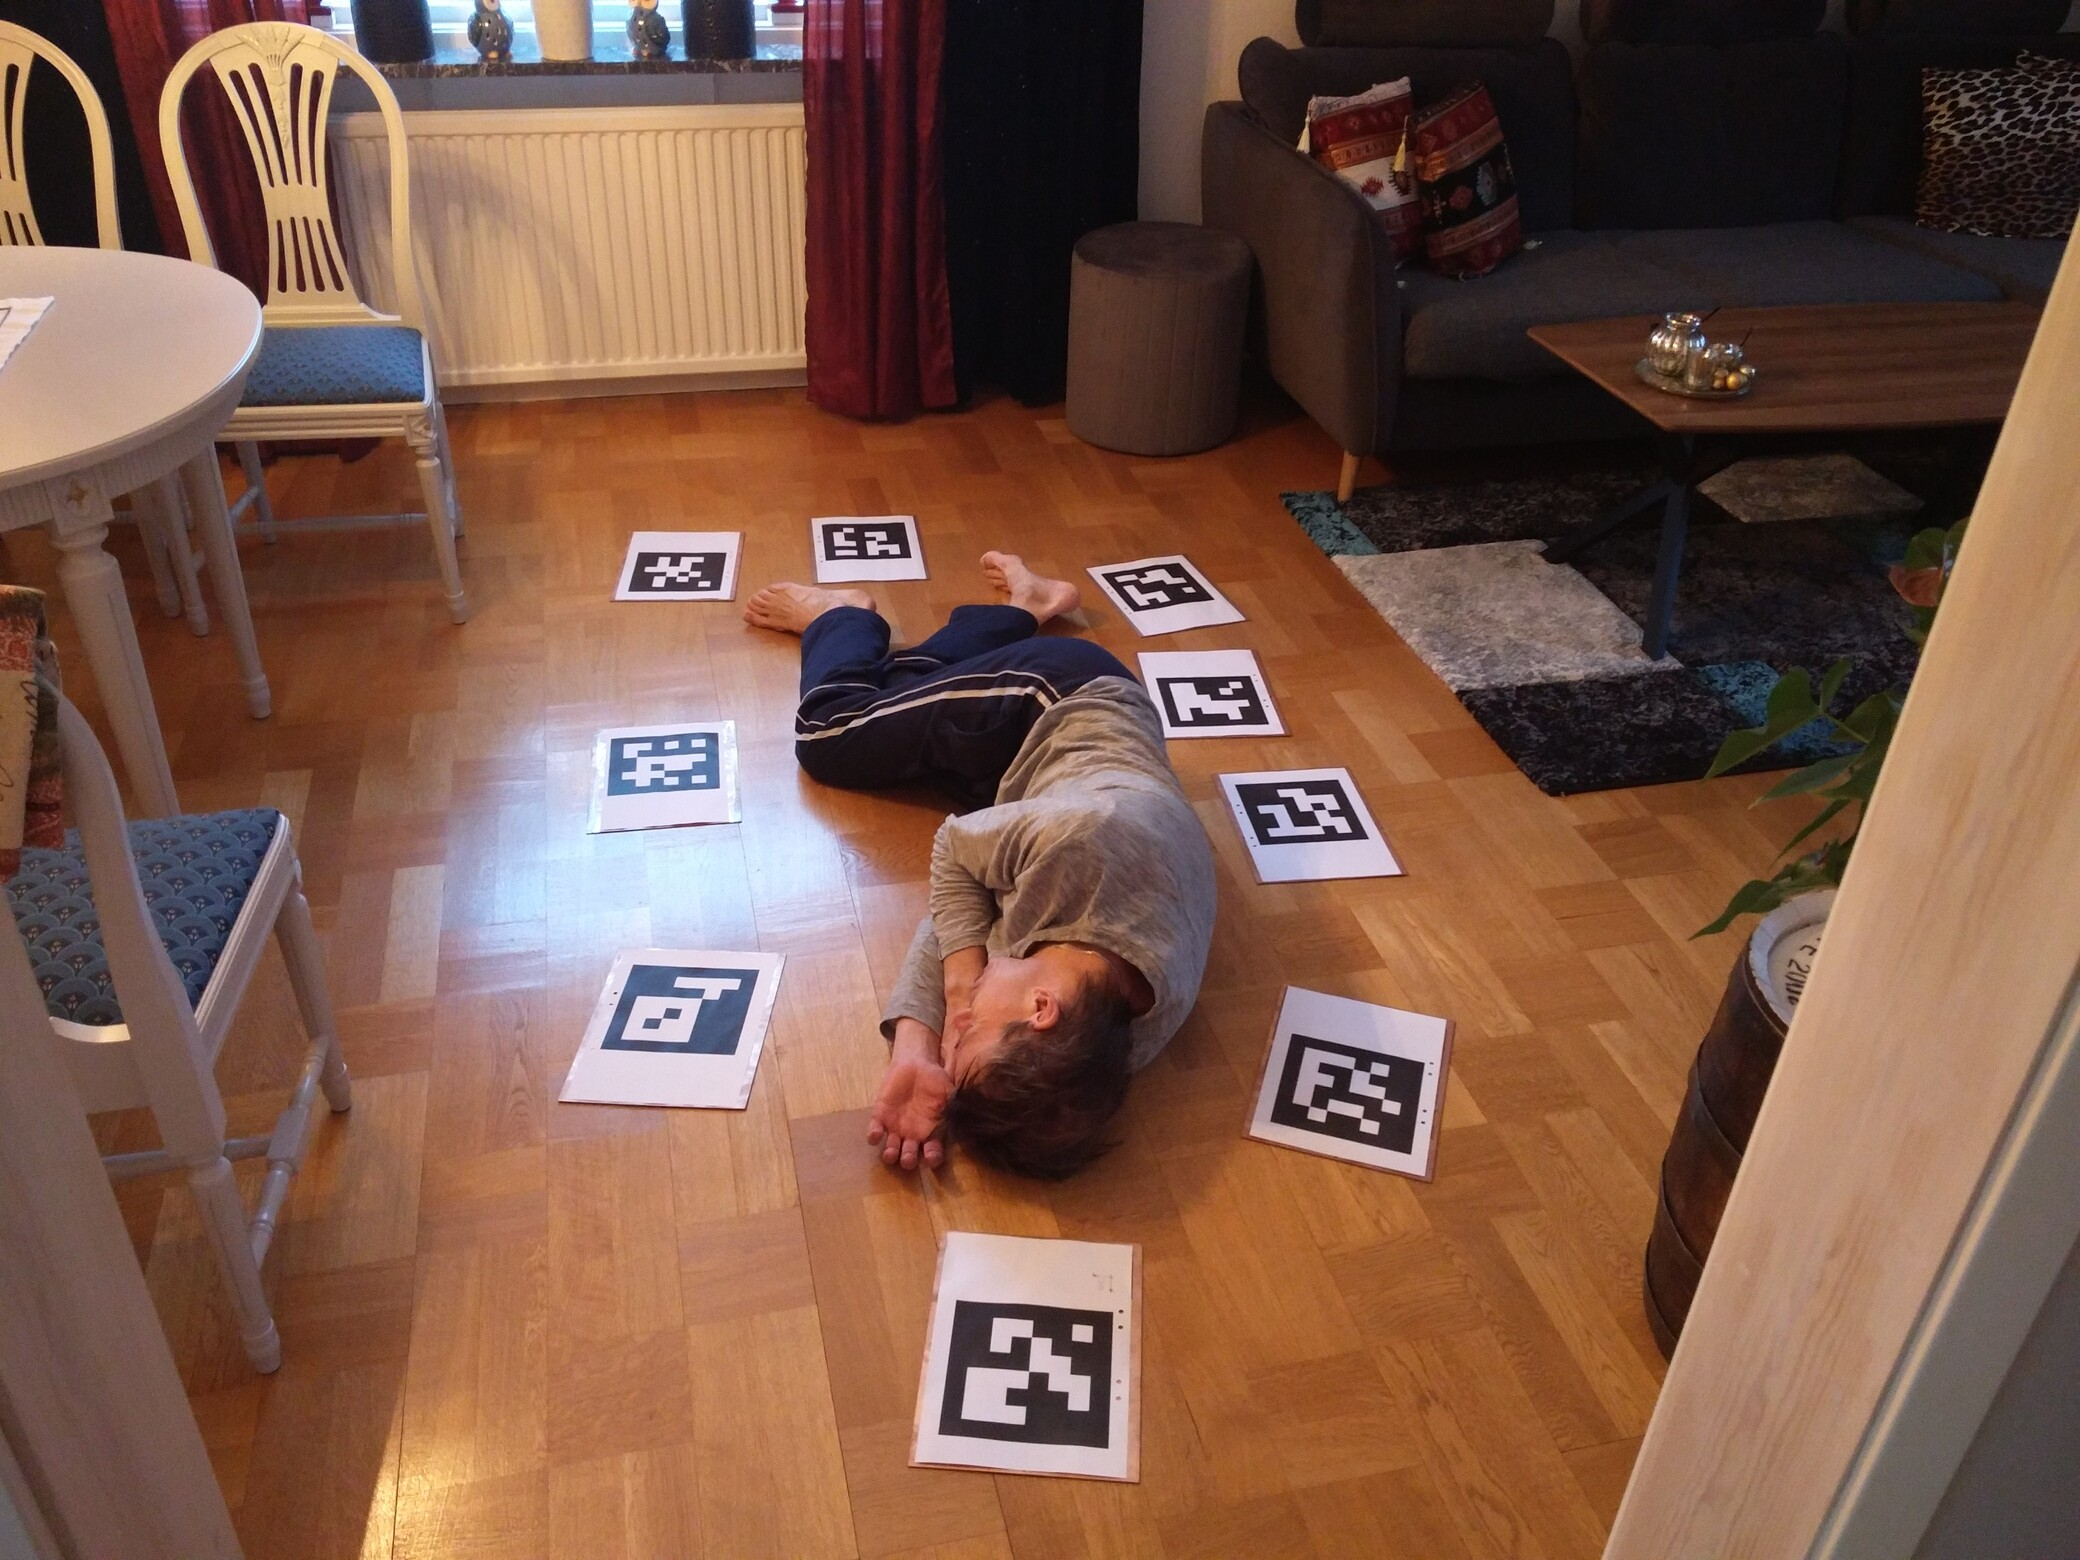
\includegraphics[width=\textwidth]{images/datasets/P2/images/093311.jpg}
        \caption*{North}
    \end{minipage}
    \begin{minipage}[t]{0.2\textwidth}
        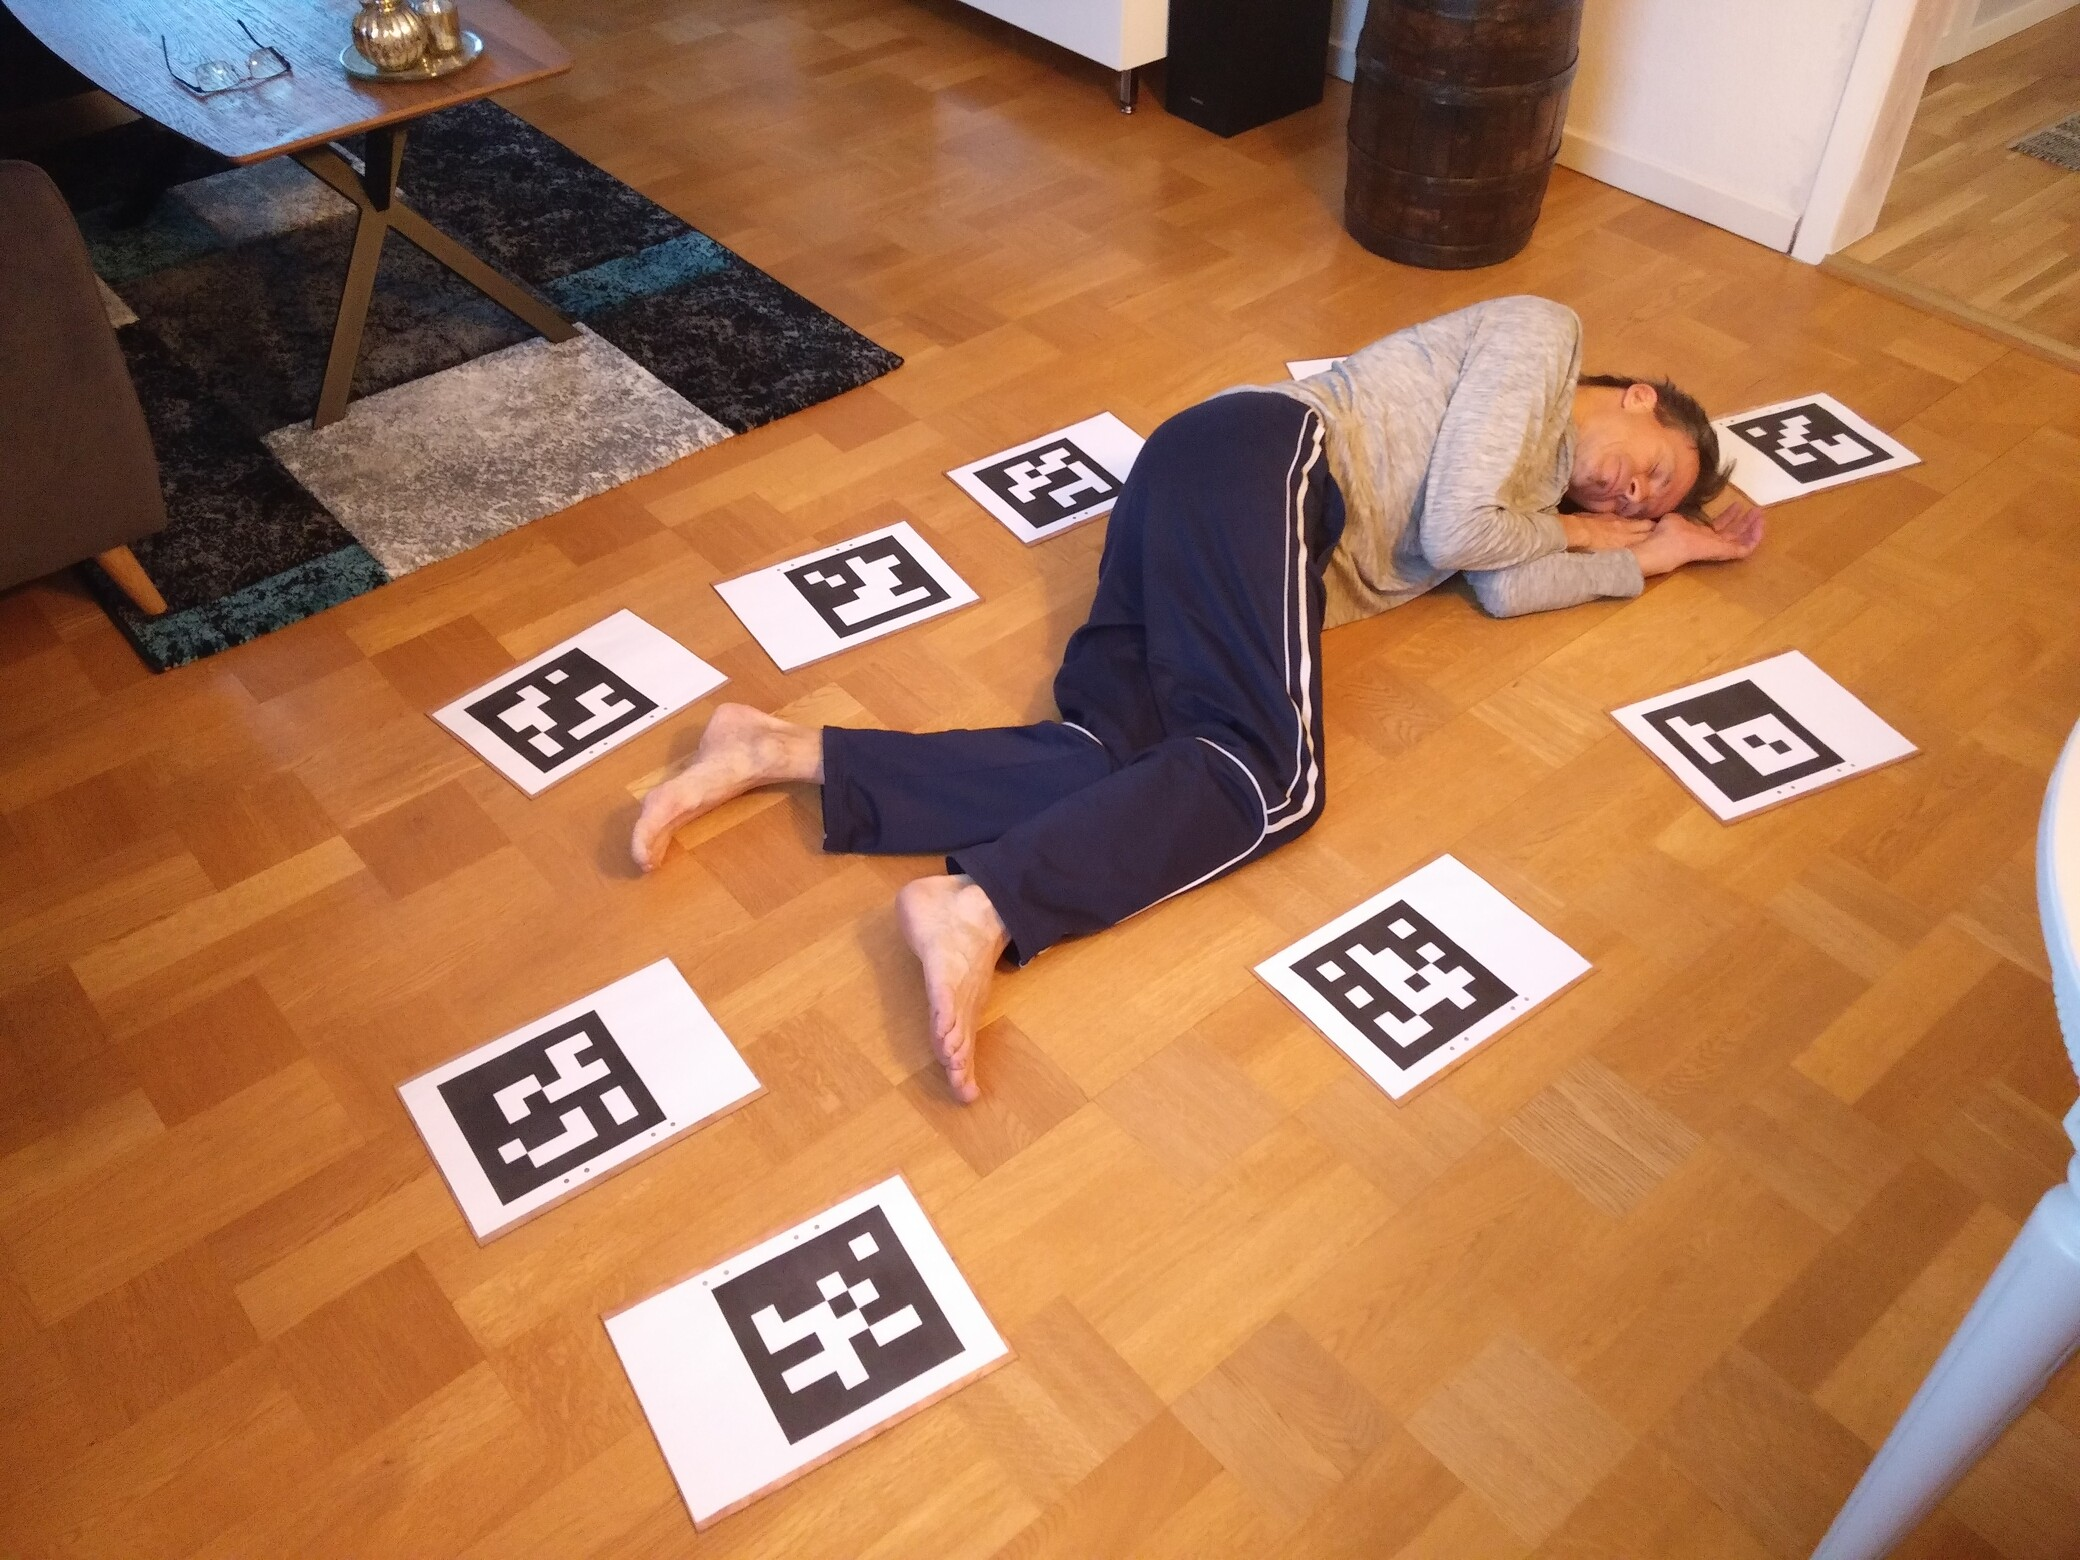
\includegraphics[width=\textwidth]{images/datasets/P2/images/093409.jpg}
        \caption*{East}
        % \includegraphics[width=\textwidth]{pic1}
    \end{minipage}
    \begin{minipage}[t]{0.2\textwidth}
        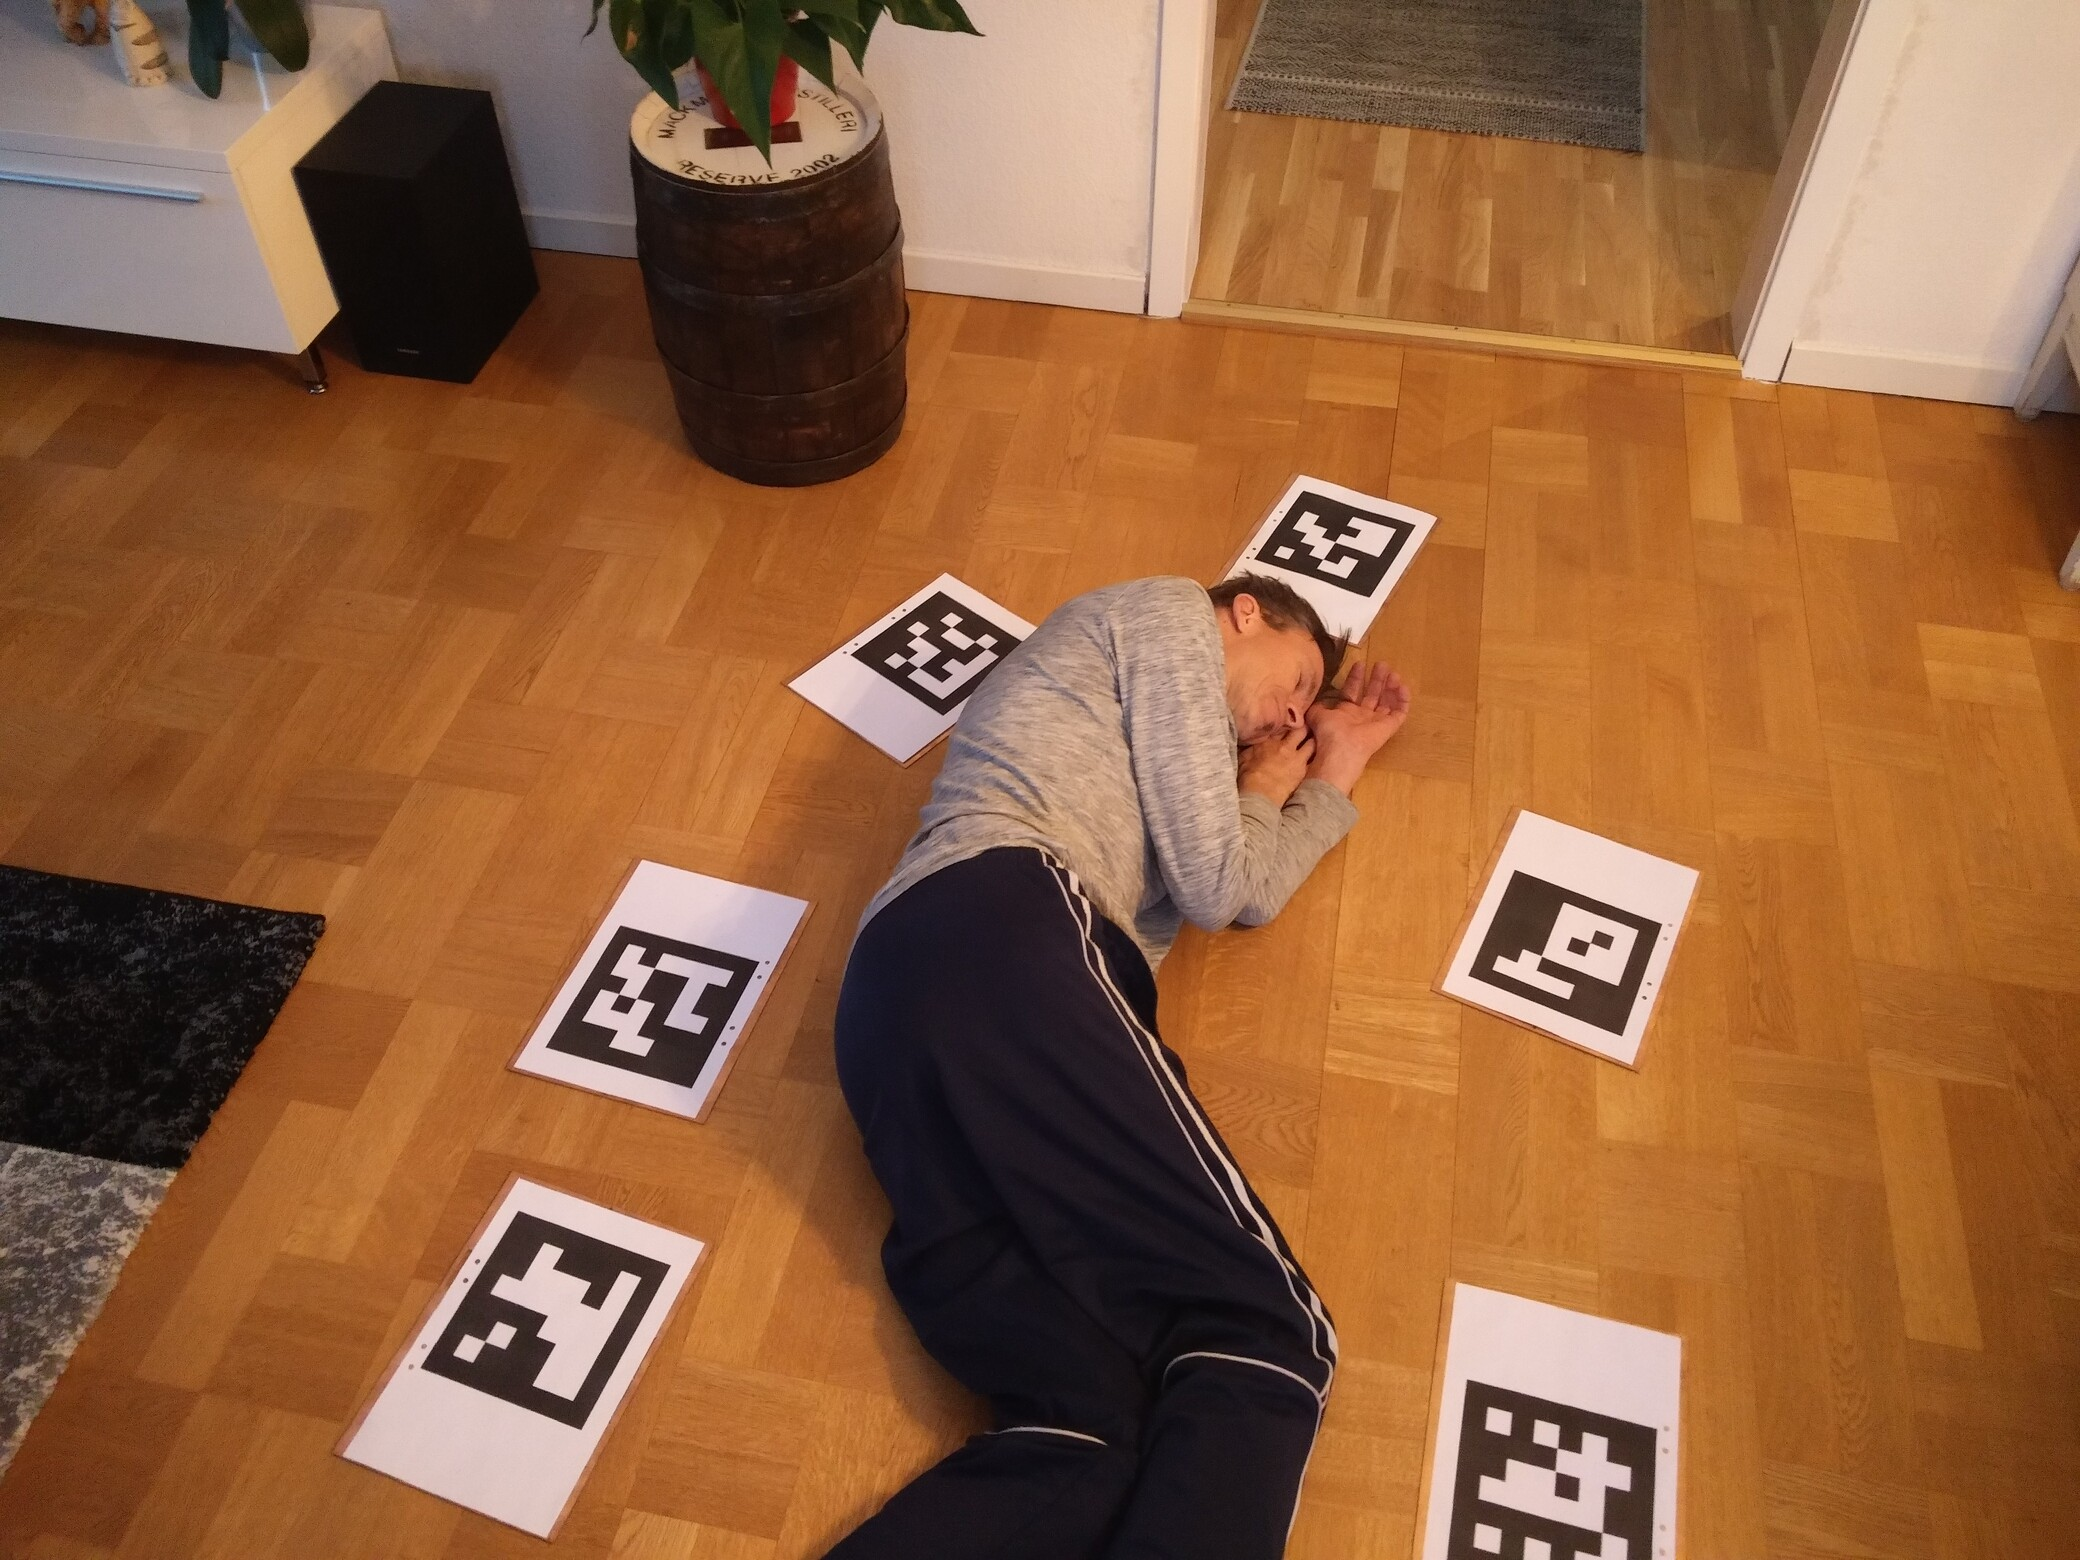
\includegraphics[width=\textwidth]{images/datasets/P2/images/093551.jpg}
        \caption*{South}
        % \includegraphics[width=\textwidth]{pic1}
    \end{minipage}
    \begin{minipage}[t]{0.2\textwidth}
        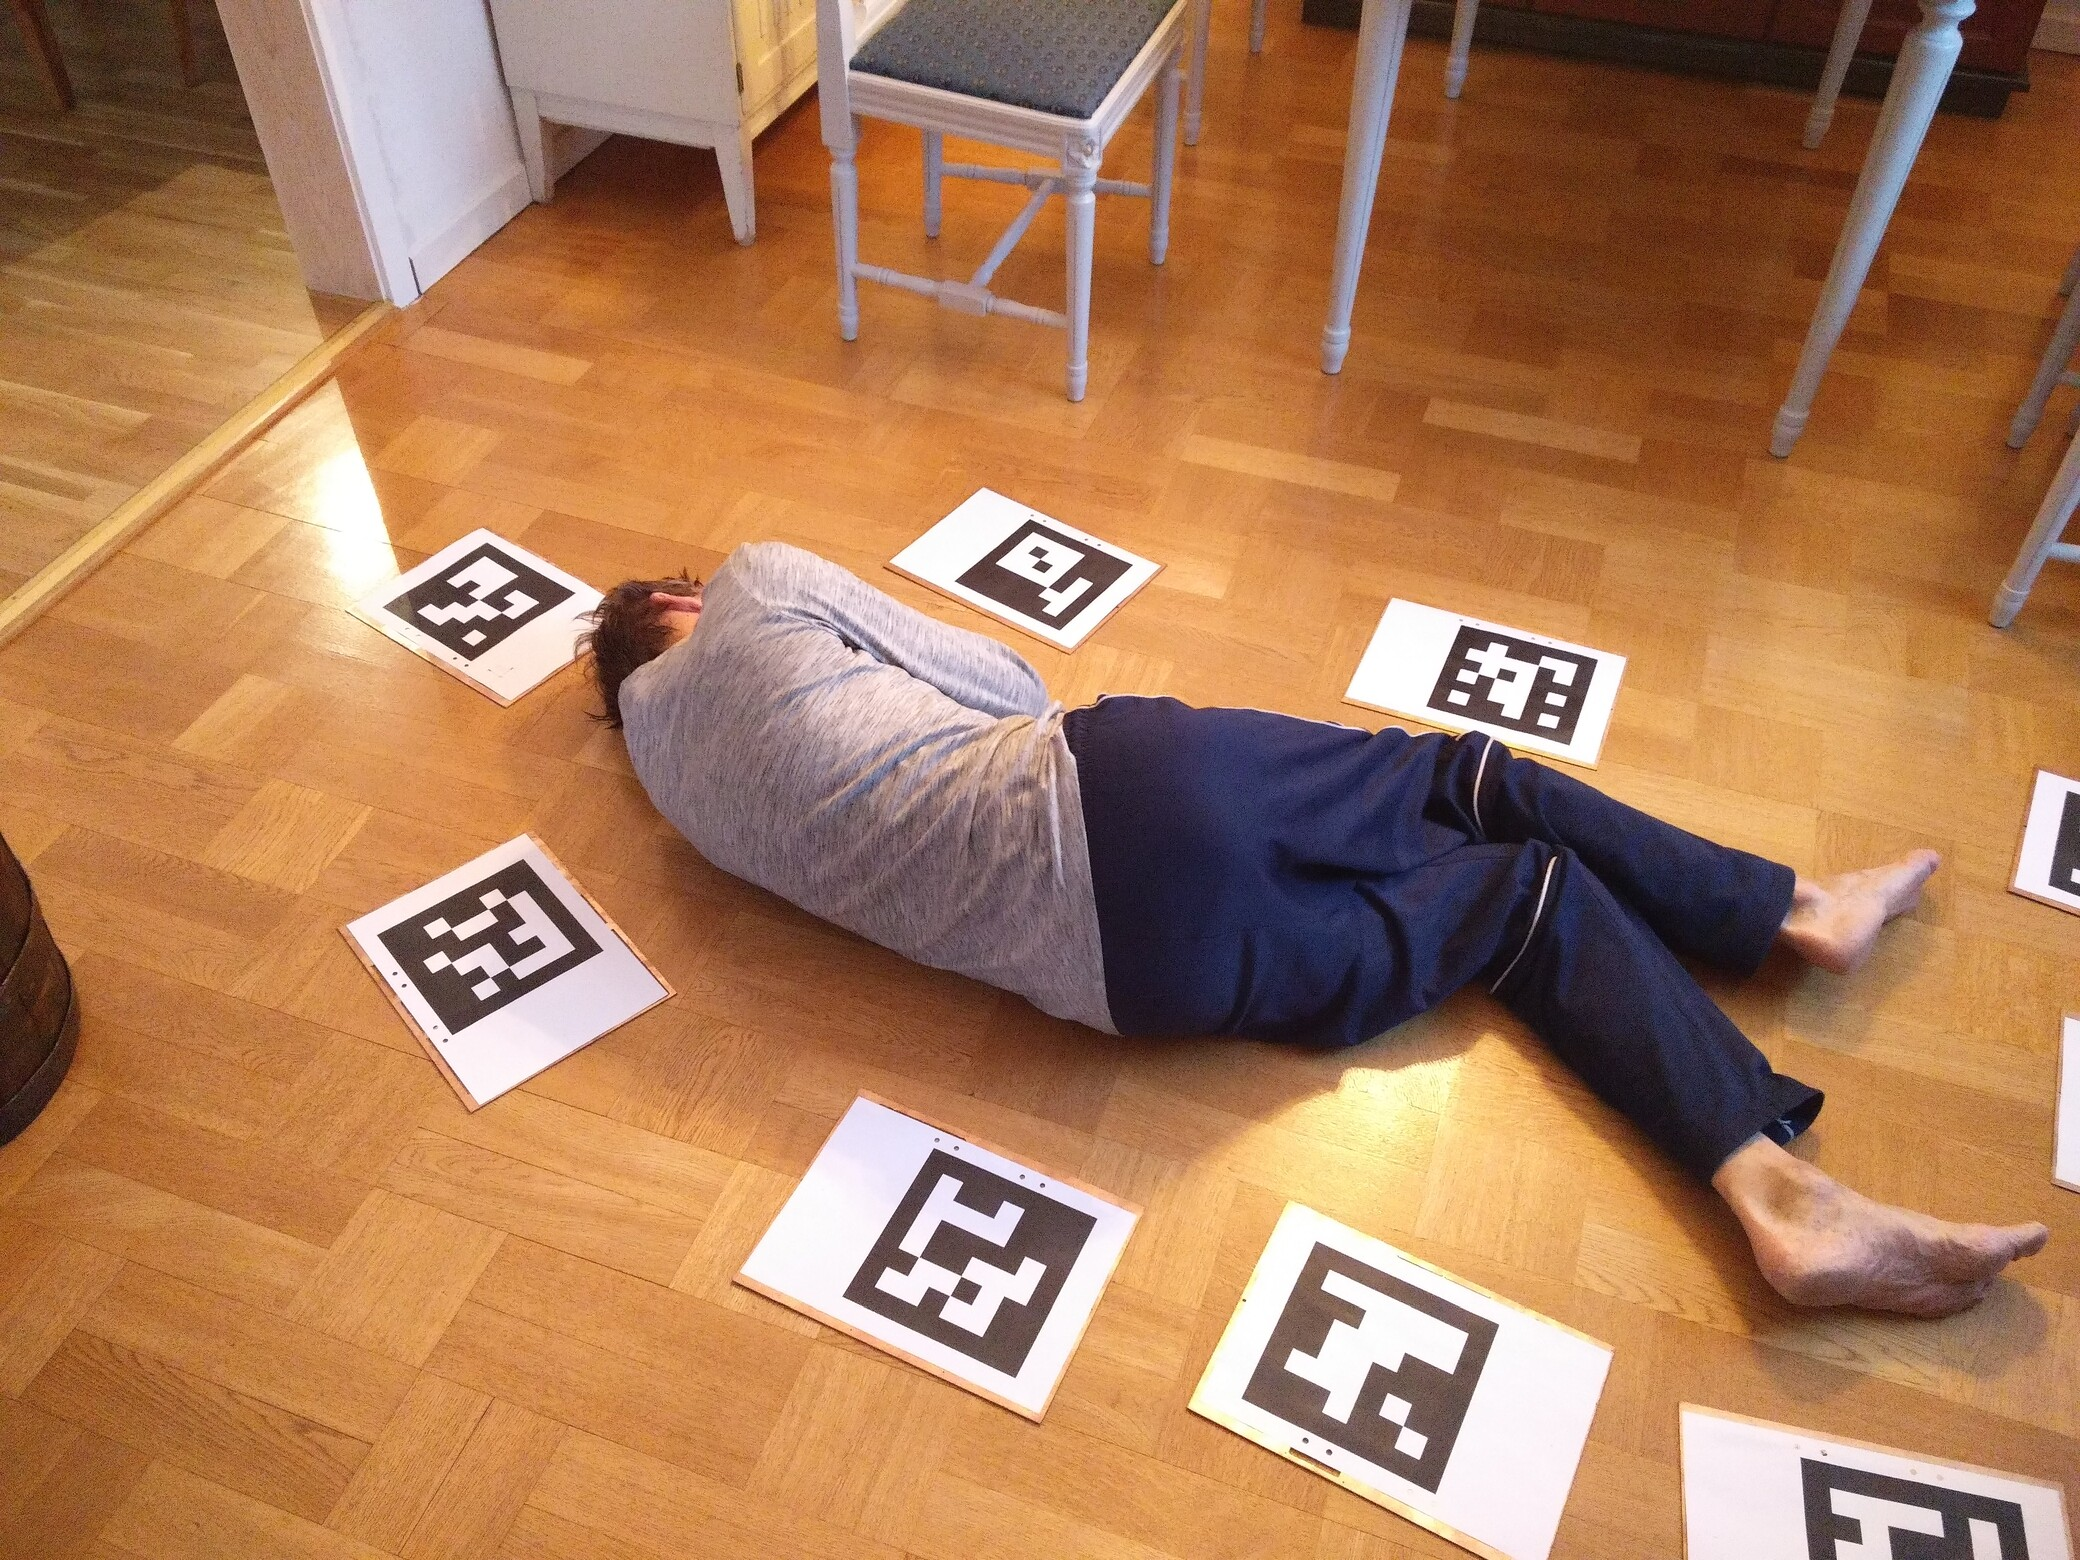
\includegraphics[width=\textwidth]{images/datasets/P2/images/093335.jpg}
        % \includegraphics[width=\textwidth]{pic1}
        \caption*{West}
    \end{minipage}
\end{center}
\caption[Camera quadrant position]{The camera quadrant position in the input set is labeled as follow.}
\label{fig:camera_pos_lables}
\end{figure}

\par

To calculate the total error for all features in every image, first use a subset to calculate the median \(\mu_{u,v}\) for each image and each feature.
Then use that to calculate the total error by taking the Cartesian distance between \(t_{u,v}\) and \(\mu_{u,v}\), who is a feature in a picture with the same label as the selected t variable.
This could be described as the Error equation
% \ref{eq:impl:muerror}.
% \label{eq:impl:muerror}

% \begin{equation} %
% \label{eq:impl:muerror}
% \mu_{error}=\frac{1}{N\cdotm}\sum_{i,j}\Bigg(\sum_{n,m}\bigg(\sqrt{(\mu_i-t_i)_x^2+(\mu_i-t_i)^2}\bigg)\Bigg)
% \end{equation}
\begin{equation} %
\label{eq:impl:muerror}
\mu_{error}=\frac{1}{M\cdotm}\sum_{i}^M\big(|\mu_i - t_1|)\big)
\end{equation}

\begin{align*}
    \text{where:}\\
    % n &= \text{ label } 1\dots N\\
    % N &= \text{ is how many labels there are in the system}\\
    % m &= \text{ image } 1\dots M\\
    M &= \text{ is how many pictures there are in the system}\\
    \mu_{i} &= \parbox[t]{7cm}{\RaggedRight is the median for a particular image,label and coordinate in the system}\\
    t_{i} &= \text{ is one feature to be tested}
\end{align*}
\par
Then the total error from OpenPose to a subset of the human set can be compared with the total error from the human set to its subset using a t-square test.
This error equation is derived from that a regular median for a one-dimensional input is
\[
\mu = \frac{1}{n}\sum_{i=1}^n (x_i)
\]
However, for a matrix, this becomes:
\[
\mu = \frac{1}{n\cdot m} \sum_{i=1,j=1}^{i=n,j=m}(x_{i,j})
\]
Then the internal \(\sum\) is just for building the matrix such that the matrix has \(n\times m\) matrix with the length from the feature to the median.





% \subsection{F-test}\label{sub:implemnt:ftest}
% Before any test can be done the variability of the selected method to test needs to be checked.
% This is done with a F-test and usually a table.
% The first part is using coagulating the ${F}_\text{calc}$
% value that is a score using the standard deviation \sigma of both samples.
% The value must be larger then 1 thus the equation becomes:

% \begin{align*}
% F_{\text{calc}} &= \frac{\sigma^2_1}{\sigma^2_2}\quad\text{if}\, \sigma^2_1 > \sigma^2_2\\
% F_{\text{calc}} &= \frac{\sigma^2_2}{\sigma^2_1}\quad\text{if}\, \sigma^2_1 =< \sigma^2_2\\
% \end{align*}

% Then after $F_\text{calc}$ is found, it needs to be compared with a value
% $F_\text{tab}$ that is usually found in a table if the calculation is done by hand, but in the case of computers, this is derived from libraries, but in this paper, it is still called $F_\text{tab}$ for simplicity.
% \par
% The value for $F_{\text{tab}}$ is derived from the dimension's of the data or how many rows there is in the table for each data set.
% So assume that there is, for example, two sets with the first set have nine rows, and the other set is seven rows. Then the dimension for the F test is $D = (9-1, 7-1)= (8,6)$.
% Using $(8,6)$ in the table \cite[p.~488]{alm2008stokastik} it can be seen that for dimension $(8,6)$ the value is $4,147$
% That means that if our $F_{\text{calc}}$ is lower then
% $F_{\text{tab}}$ then the results are statistically similar to each other.
% That result can then be used to determine if the variance $\sigma$  is equal in both sets, which then determines the t-test category.

% \subsection{T-test}\label{sub:implement:ttest}
% The t-test is a set of tests that will differ based on what data represents.
%\begin{figure}
%    \centering
%    \scalebox{.4}{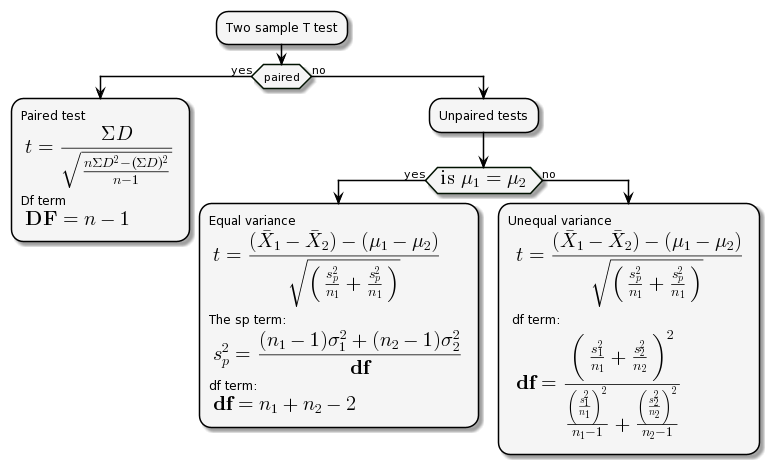
\includegraphics{images/selecting_t_test.png}}
%    \caption{Selecting t test}
%    \label{fig:impl:select_t_test}
%\end{figure}

% \subsection{Verifying the algorithm}%
% \label{sub:Verifying_the_alorithm}
% To verify that the algorithm works as intended, a smaller set of images containing measurable features.
% In this set, it proposed to include a large checkerboard and a few spheres of bright colours to be used as features, and the camera can be mounted to a bracket to be able to intensify the exact location.
% In figure~\ref{fig:validations} a short overview of the system is shown.



% % \def\svgwidth{\columnwidth}
% \begin{figure}[ht]
%     \centering
%         \input{images/validation.pdf_tex}
%         % \input{Figures/validation.pdf_tex}
%       \caption{
%           to be directed in different directions.
%           Future more the tree \aruco corners in the image, scatted on the floor.
%           Also, observe that the \aruco corner $A_0$ can not be followed by camera $C_2$; thus, the camera's position can not be derived directly from $A_0$.
%           However, the position of $C_2$ can be derived by using transfer matrices from the other cameras.
%           In this image, two features marked as $F_g$ and $F_r$ are also present and will be used to validate the system by using the marked checkerboard floor to indicate where the features are in the real world.
%           If the system generates the same features concerning $A_0$ with some scaling factor $\alpha$, the system is valid.
%       }
%     \label{fig:validations}
% \end{figure}


% \begin{figure}
% \begin{center}
%     \includegraphics[width=10cm]{images/uml_outline.pdf}
% \end{center}
% \caption{This figure describes the outline of the project using UML as output layer. At the top the camera with its matrix is shown while the map in the in the bottom is the relation between \aruco corners and camera pose}
% \label{fig:UML_outline}
% \end{figure}



 %SOTA
\newpage
\section{Related Work}
\label{sec:related_work}
In this paper, an evaluation of accuracy is performed on subjects lying on the ground is preformed from several angles with body parts partly occlusion because it remains hidden under the body.
This occlusion can pose a problem for methods that uses a model-based/top-down approach mentioned by Sarafianos et al. ~\cite{sarafianos2016} with a pre-defined skeleton as suddenly the images have a missing body part due to self-occlusion.
Future more the according to Sarafianos, the top-down approach takes significantly more time to compute than a generative bottom-up model.
%But the bottom line is that pose estimation from a monocular camera requires heavy computation for each frame.
Sins machine learning is the primary method for solving this problem; a god data set is necessary.
Currently, at the time of writing, there exist no 3D pose dataset for humans that are lying on the ground outside the lab environments \cite{yang2018, mehta2017, yasin2016, wang2019}.
However, in late 2020, a new paper with a set of images with humans laying in beads was released by Liu et.al\cite{liu2020simultaneously}, thus laying the groundwork for starting a set where the subject is laying down.
This set was named \ac{slp} with includes 109 participant S lying in a bed.
The set then contains images taken with an \ac{rgb} camera, \ac{rgbd} camera with depth information, \ac{lwir} camera and a pressure mat.
In the broader perspective, Erika D’Antonio et al. \cite{d2021validation} evaluates the accuracy of \openpose{ } when the subject is walking by observing the joint angles between each joint.

% Slam navigation.
%To accurately reconstruct 3D geometry, a camera pose estimation method is used.
Camera pose estimation is commonly used in robotics and \ac{vr} to determine the 3D dimensional position of either the player or the robot.
To to solve this problem according to Mu{\~n}oz-Salinas et.al\cite{munoz2018mapping} a great part of the research focus on \ac{sfm} and \ac{slam}.
However, Mu{\~n}oz-Salinas continues, keypoint matching has a somewhat limited invariability to scale and rotation, which can make the method unable to find a solution.
In their work, they instead divide up the tasks into three steps, mapping the markers in the input domain, creating a pose quiver for how each marker is connected, and finally calculating each marker's global position and camera using the shortest path algorithm.
Nevertheless, they refine the position by solving the bundle adjustment problem to fine calibrate the position.

%aruco markers and aruco mapping
% reliable markers \cite{garrido2014automatic}
% Mapping and localization from planar markers \cite{munoz2018mapping}


\newpage
\section{Method} 
\label{sec:method}
As \openpose is only trained on humans standing, walking, running and sitting.
The assumption in this paper is that \openpose is bad at humans on the ground.
But is that true or not?
If openpose is as good as a human at identifying where each feature on the human is located in both 2D and 3D, then a hypothesis formed such that the median and variance of both human and open pose should be equal.
$$
\text{H}_0\quad \mu_{human} = \mu_{OpenPose} \quad\text{AND}\quad \sigma_{human} = \sigma_{OpenPose}
$$
$$
\text{H}_1\quad \mu_{human} <> \mu_{OpenPose} \quad\text{OR}\quad \sigma_{human} <> \sigma_{OpenPose}
$$


The test is done in both 2D and 3D with a minimal error method using \aruco corners.
In the end, the 3D method did not work, but sufficient validation for the hypothesis was derivable from the 2D position.
To prove the claim that OpenPose was unable to find the human features accurately.
A F-test for testing the variance and a T-test for testing the median is performed on data that is derived both from several collected data points from both human and OpenPose.






\newpage
% 
\section{Implementation}
\label{sec:work}

This research implemented the code using Python due to its vibrant echo system of predefined packages already available in its package database.
The overall implementation is described in figure~\ref{fig:project_overview} that describes how users annotate the data taken from images on the subject in the scene and how that leads to the results given in~\ref{sec:results}.
As can be observed, the system is implemented as a "one-shot" static implementation that first collects images in a prepossessing step.

In the prepossessing step, images are loaded in 1.0 and camera annotations 1.2.
The images are annotated in 1.9 by both humans\footnote{Using \url{https://www.makesense.ai/}} and in 1.1 by \openpose{ }.

Figure~\ref{fig:1.1.openpose_anotation} shows how \openpose{ } works with the system to create the annotations for the features in the image and how it is saved to disk as a \ac{csv} file.
The figure~\ref{fig:1.6.feoture_antotation} shows how that data saved in multiple \ac{csv} files are combined in to one database accessible from a class-based \ac{api}
This \ac{api} can be used find relations between users and \openpose{ } or even camera directions.

Then after that, the implemented system is explained in the system part, where 3D reconstruction 1.4 is of particular interest, and figure~\ref{fig:1.4.3D_reconstrution} provides a deeper explanation.

Figure~\ref {fig:1.3_input_statistics} shows how the input from both the camera quadrant annotation and features is annotated.
Of specific interests is 1.3.6 and 1.3.7, they split the data into multiple tables that, for example, 1.3.7 returns for tables, one for each quadrant north, east, south and west.
1.3.4 (a,b) uses equation\ref{eq:impl:muerror} to calculate the median error for that feature with regards to the median of the user group.




\begin{figure}[ht]
\begin{center}
    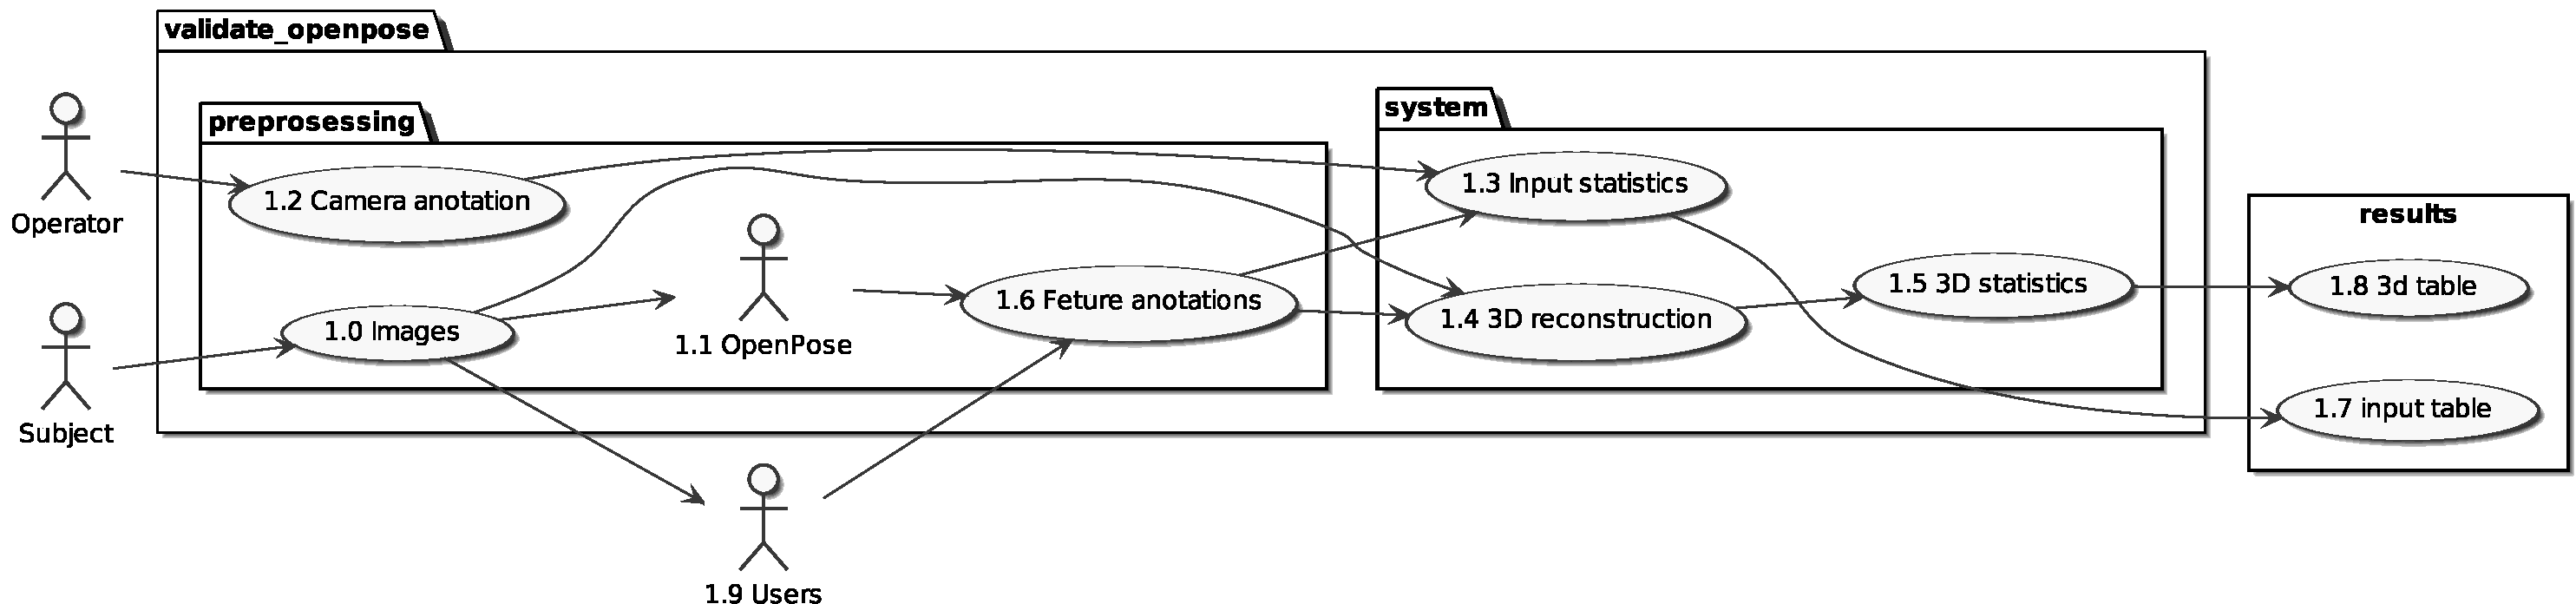
\includegraphics[width=0.9\textwidth]{figures/project_overview.png}
\end{center}
\caption[Project Overview]{In this figure, the overall intended implementation of the system. The subject is the person on the floor while users are the one who annotates the images. The general camera quadrant where the camera was located is annotated by the Operator who took the images. In this image \openpose is displayed as a human, but that is only for clarity that the images are supposed to be annotated equally by both user and \openpose. 1.0 images are stored on the computers file system and can be accessed using Python.}
\label{fig:project_overview}
\end{figure}


\begin{figure}[ht]
\begin{center}
    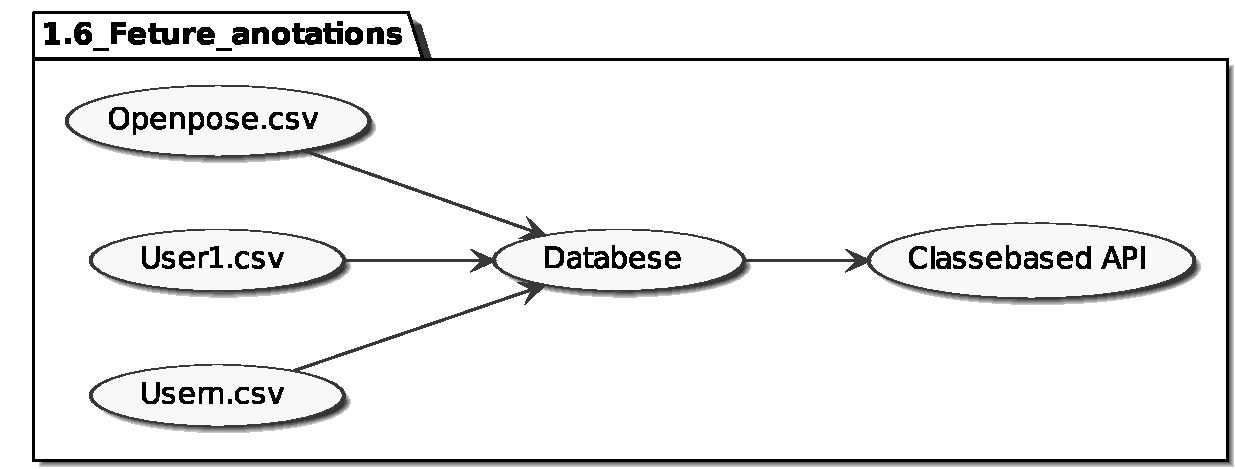
\includegraphics[width=0.3\textwidth]{figures/feature_anotation.png}
\end{center}
\caption[1.6 feature anotations]{In figure~\ref{fig:project_overview} the block 1.6 Feature Annotations to from \ac{csv} build a database and create an class based API that then 1.3 and 1.4 then uses to future create the validation system. Note that \openpose{ } is only one entity while there are n many users}
\label{fig:1.6.feature_antotation}
\end{figure}



\begin{figure}[ht]
\begin{center}
    
\includegraphics[scale=0.4]{figures/openpose_anotation.png}
\end{center}
\caption[1.1 OpenPose anotations]{In this figure the implemented step of 1.1 in figure\ref{fig:project_overview} shows how \openpose takes in images and convert annotate, convert and save the annotations as a CSV file.}
\label{fig:1.1.openpose_anotation}
\end{figure}




\begin{figure}[ht]
\begin{center}
    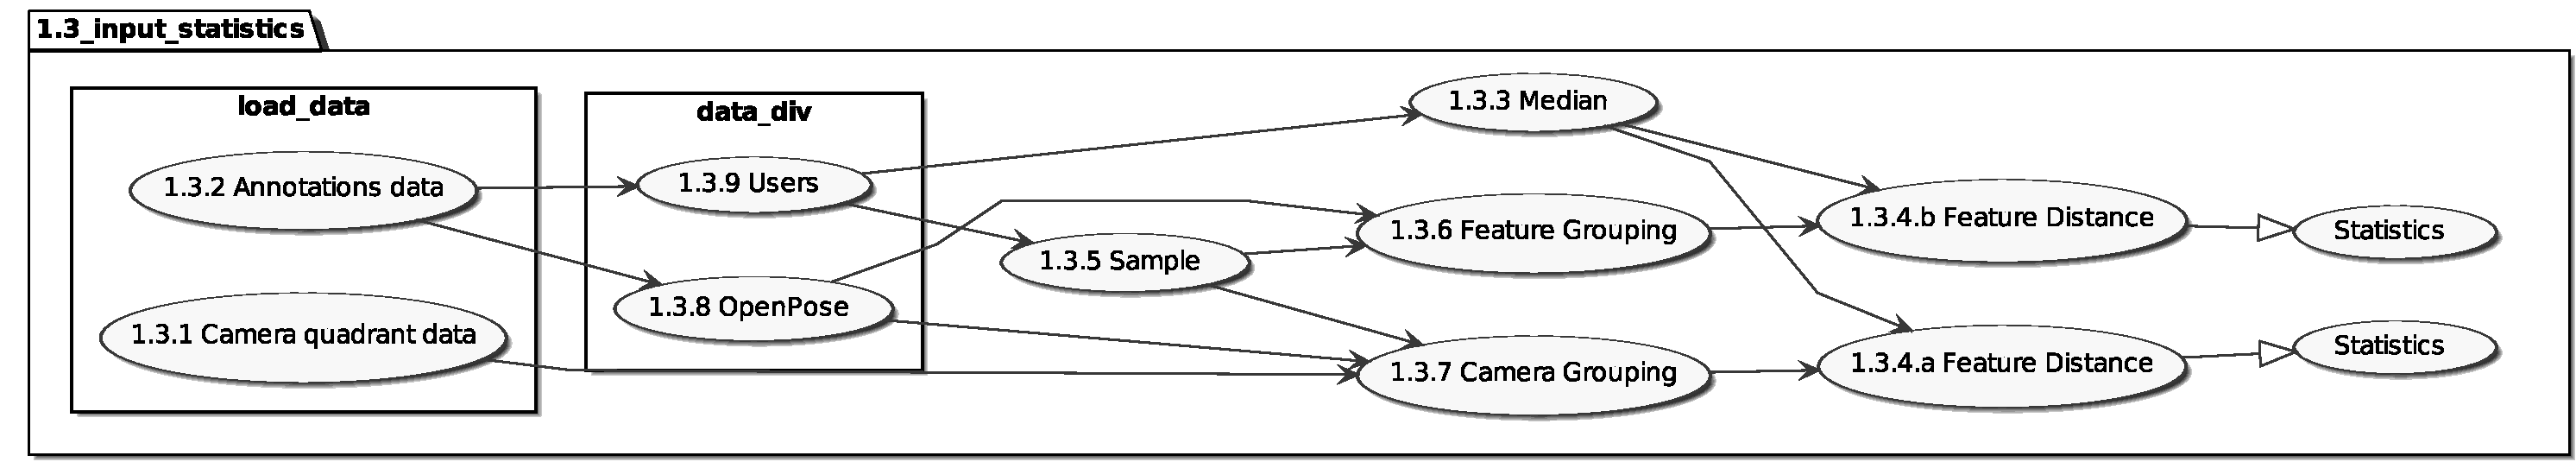
\includegraphics[scale=0.3]{figures/input_statistics.png}
\end{center}
\caption[1.3 Input statistics]{From block 1.3 in figure~\ref{fig:project_overview}, This figure shows how the input data is processed 1.3.2 loads the annotated data while 1.3.8 and 1.3.9 splits the data up in \openpose and users. 1.3.5 a sample is drawn and the rest of the data makes the 1.3.3 median. 1.3.6 Feature grouping is organising the data according to its features while 1.3.7 organises the data according to Camera quadrant. In 1.3.4 (a,b) the distance equation~\ref{eq:impl:muerror} to calculate the distance from annotated data.}
\label{fig:1.3_input_statistics}
\end{figure}

\begin{figure}[ht]
\begin{center}
    \includegraphics[scale=0.26]{../figures/3D_reconstrution.png}
\end{center}
\caption[1.4 3D reconstruction]{In thins figure the general function for 3D reconstruction is presented. 1.4.1 Load the camera 3D position and how that works is presented in figure\ref{fig:1.4.1_camerapose}. 1.4.2 loads the features for the 2D features on each image. 1.4.3 represents the majority of the human answers while 1.4.4 Is the minority sample. 1.4.5 is the \openpose feature response. 1.4.6 (o,h and s) is the projective geometry deeper explained in figure~\ref{fig:1.4.6.proj_geometry}. 1.4.8 creates a median $\mu$ constructed form the 3D point cloud in 1.4.6.h. 1.4.9 and 1.4.10 Calculates the distance from the median generated in 1.4.8 and the results are sent to the statistics module~\ref{} }
\label{fig:1.4.3D_reconstrution}
\end{figure}

\begin{figure}[ht]
\begin{center}
    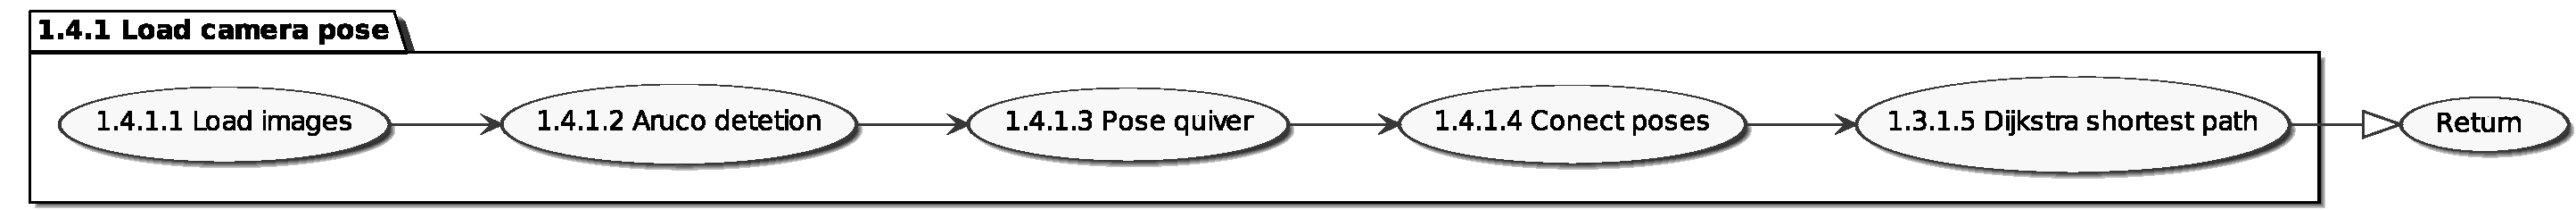
\includegraphics[scale=0.3]{../figures/camerapose.png}
\end{center}
\caption[1.4.1 Camera pose]{From figure~\ref{fig:1.4.3D_reconstrution} the position of the camera is calculated in the following steps. 1.4.1.1 Loads the images from the database, 1.4.1.2 Aruco detection detects each individual \aruco in each image and provides the transfer matrix from the camera to the \aruco corner. In 1.4.1.3 the pose quiver connects each corner to each corner in each image figure~\ref{fig:trans_calc} shows the process for that a bit deeper. 1.4.1.4 connect the corner to each corner using the algorithms in~\ref{sub:implement:relative}. 1.4.1.5 Dijkstra is used to derive shortest path from each corner to corner and corner to camera with the position of each step saved in each corner/camera}
\label{fig:1.4.1_camerapose}
\end{figure}


\begin{figure}[ht]
\begin{center}
    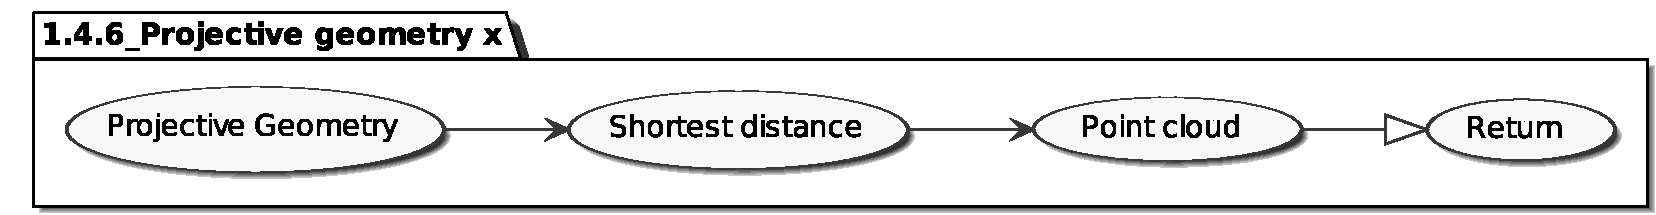
\includegraphics[scale=0.35]{../figures/proj_geometry.png}
\end{center}
\caption[1.4.6 Projection geometry]{The projective geometry in figure~\ref{fig:1.4.3D_reconstrution} 1.4.6 (o,h and s) is shown in this figure how first the node projective geometry using the calculations in~\ref{sub:Midpoint} to calculate the projective line out of the camera through a feature from ether \openpose or a human. Shortest distance is the distance between ether two ore more lines for each image and each feature, visually demonstrated in figure~\ref{fig:3Dhuman}. This generates a point cloud with point for each shortest distance.}
\label{fig:1.4.6.proj_geometry}
\end{figure}




Those corners are then identified and connected such that the corner nr 1 in image one is connected to corner nr 1 in image 2.
This process builds a pose quiver of how each corner is connected to each image.
With that process done, the \aruco{ } library can generate the $\vec{t}$ and $\vec{r}$ that determines the camera concerning that corner.

However, it is not as explained in\ref{sub:implement:relativepath} the path from the \aruco to the camera that is interesting.
Instead, the pose quiver calculates the path from origin to the camera using transfer matrices.
% This is done by using Dijkstra's algorithm for the shortest path and then the algorithm~\ref{alg:inverse},~\ref{alg:relative}
%On the implementation side, this is done by first calculating the path from the origin to the camera using Dijkstra's algorithm.

On the implementation side, the first step in the code is calculating the cumulative transfer matrix from origin to each corner by first setting the origin as $I$.

\input{figures/trans_calc.latex}



% \newpage
\section{Ethics}
\label{sec:ethics}

%I först hand avser vi med ”etik” här forskningsetiska frågor. Innebär ditt val av frågeställning eller metod något forskningsetiskt ställningstagande? Om du till exempel intervjuar personer för ditt arbete, kan du garantera dessa anonymitet och på vilket sätt använder du den information du får av dem? Finns det andra etiska aspekter att beakta i arbetet? Kan det finnas etiska aspekter på resultatet av ditt arbete? Du bör tydligt ange om du anser att ditt arbete inte innehåller några forskningsetiska frågor.

%Du ska också kritiskt granska och analysera ditt arbete med hänsyn till samhälleliga aspekter. Här kan du till exempel diskutera hur ditt arbete förhåller sig till mål som ekonomisk, social och ekologiskt hållbar utveckling. Det kan också finnas juridiska och politiska aspekter på ditt arbete.
According to Starrett, Steve in \cite{starrett2017engineering} the engineer should consider un-ethical use of the implemented system's.
Thus in this part, the system is broken up into previously discussed parts of vision and the robot itself as each faeces different ethical considerations.
As this work uses images of actual humans, the risk is that a picture used in this work is used maliciously.
Other than that, there are no primary ethical considerations for this work.
\newpage
\section{Results}\label{sec:results}

%Här kan du till exempel presentera resultat av experiment, bevis, analys av data etc. Dina resultat måste beskrivas så tydligt att en läsare kan bedöma dem.  Du ska också förklara och analysera resultaten.

The results so far is divided up in two relevant subsections where the first handles the input inference test and the second handles the 3D reconstruction using \aruco corners.
\subsection{OpenPose output inference results}%
\label{sub:res:op_inference}



%----------------------------
\begin{table}[htb]
    \begin{center}
    \begin{minipage}{0.4\textwidth}
        \begin{center}
            \input{../results/error_degdf_df.latex}
        \end{center}
        \caption{The degrees of freedom for human and \openpose is due to the quite limited dataset not in most cases not statistically viable but perhaps it cold work as a marker.}
        \label{tab:results:degfreedom}
    \end{minipage}
    \begin{minipage}{0.4\textwidth}
        \begin{center}
            \input{../results/direction_degdf_df.latex}
        \end{center}
        \caption{The directional degrees of freedom is a bit better because it do not care about the labels, just the total error for that direction. }
        \label{tab:results:dirdegfreedom}
    \end{minipage}
    \end{center}
\end{table}
%----------------------------
\begin{table}[htb]
    \begin{center}
        \input{../results/ftest_pos_df.latex}
    \end{center}
    \caption{The directional results from F-test and T-test}
    \label{lab:results:human_lable}
\end{table}
%----------------------------
\begin{table}[htb]
    \begin{center}
        \input{../results/error_df.latex}
    \end{center}
    \caption{The error results for the human vs \openpose in the image domain. Observe the large variance in the forth column that suggests that \openpose have problem finding the correct solution for that label. It can also be observed that the half of the data in comparison with the human is missing from \openpose columns thus indicating again that it could not find a solution to that label.}
    \label{lab:results:human_vs_openpose}
\end{table}
%----------------------------


\subsection{3D reconstruction using Aruco}%
\label{sub:res:3drec}
\begin{figure}
\begin{center}
    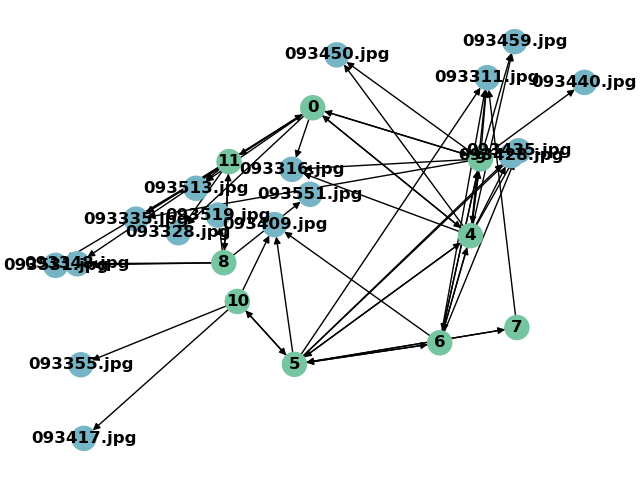
\includegraphics[scale=0.6]{results/atlas.png}
\end{center}
\caption{Reconstructing the map for the input data proved to be a harder problem then initially thought. Ni this results the green numbered nodes seams to find the correct location, but the input camera view nodes in blue do not.}
\label{fig:results:mapreconstruction}
\end{figure}




\newpage
\section{Diskussion (Discussion)}

Här presenterar du tolkning av resultaten och bedömer deras signifikans. Diskutera möjliga konsekvenser av resultaten, och presentera eventuella rekommendationer. Det är viktigt att du redogör för om du uppnått de mål du satte upp och därmed besvarat din frågeställning och uppnått syftet med arbetet. Avsnittet ska också innehålla reflektioner kring arbetet, som till exempel dess begränsningar.  Du kan också diskutera lösningar på problem som du identifierat och diskuterat tidigare, eller ta upp andra problem som arbetet inte behandlat, frågor som ej besvarats. Koppla också dina resultat till tidigare arbeten. På så sätt kan diskussionen bli ett samtal med det du skrev i tidigare avsnitt.  Slutligen ska du sätta ditt eget arbete i ett större sammanhang, bredda ditt perspektiv. Kan dina resultatet generaliseras? Kan det du gjort användas i något annat sammanhang? 

\newpage
\section{Slutsatser (Conclusions)}

I detta avsnitt ska du summera rapporten samt presentera slutsatser och slutanalys. Ge en kort översikt av syftet och frågeställningen. Du ska sedan tydligt tala om de viktigaste resultaten, förklara deras signifikans och sätta in dem i sitt sammanhang. Alla slutsatser ska ha stöd i tidigare delar av rapporten.  Du ska däremot inte presentera nya detaljer. 

En expert ska kunna läsa detta avsnitt oberoende av resten av rapporten. 


\newpage
%%\input{sections/Acknowledgments}
%% ============================= References ============================
%%% \newpage
\printbibliography
\addcontentsline{toc}{section}{References}

%% ============================ Appendices =============================
\newpage
\begin{appendices}
    \section*{Appendices}
    \label{sec:appendices}
    % \input(sections/99_appendix.tex)
    text

	
\begin{landscape}

\begin{table}[]
    % {\resizebox{10cm}{!}{
        \begin{center}
            \tiny
            \addtolength{\tabcolsep}{-2pt}
        \input{../results/human_error_df.latex}
        \end{center}
    % }}
        \caption{Human error}
    \label{tab:apx:human_error}
\end{table}
\begin{table}[]
    % {\resizebox{10cm}{!}{
        \begin{center}
            \tiny
            \addtolength{\tabcolsep}{-3pt}
        \input{../results/openp_error_df.latex}
        \end{center}
    % }}
        \caption{OpenPose error}
    \label{tab:apx:openp_error}
\end{table}





% % Last on this side
\end{landscape}

	\clearpage
    \input{results/datasets.latex}

	%\input{appendices/appendices2}
	\clearpage
    
\begin{algorithm}
    \caption{Inversing tvec and rvec using Rodrigues transforms}\label{alg:inverse}
    \begin{algorithmic}[1]
        \Procedure{inversePerspective}{rvec, tvec}
        \State $\vec{t} \gets tvec$
        \State $R \gets Rodrigues(rvec)$ \Comment{Vector to matrix}
        \State $R \gets matrix(R)^{T}$ \Comment{Array to transposed matrix}
        \State $\vec{t}^{-1} \gets R \cdot matrix(-\vec{t})$ \Comment{Dot product}
        \State $\vec{r}^{-1} \gets Rodrigues(R)$ \Comment{Rodrigues again}
        \State \textbf{return} $\vec{r}^{-1}, \vec{t}^{-1}$ \Comment{Matrix to vector}
        \EndProcedure
    \end{algorithmic}
\end{algorithm}



\begin{algorithm}
    \begin{algorithmic}[1]
        % \Procedure{relativePosition}{$\vec{t_1}$, $\vec{r_1}$, $\vec{t_2}$, $\vec{r_2}$}
        \Procedure{relativePosition}{rvec1,tvec1,rvec2,tvec2}
       % \Procedure{inversePerspective}{r, t}
        \State $\vec{r_1} \gets reshape(rvec1, (3,1))$ \Comment{Reshape the vectors}
        \State $\vec{t_1} \gets reshape(tvec1, (3,1))$
        \State $\vec{r_2} \gets reshape(rvec2, (3,1))$
        \State $\vec{t_1} \gets reshape(tvec2, (3,1))$
        \State $\vec{r}^{-1}, \vec{t}^{-1} \gets InvercePrespective(\vec{r}, \vec{t})$
             \Comment{Inverse the second marker}
        \State $\text{comp} \gets composeRT(\vec{r_1}, \vec{r_2}, \vec{r}^{-1}, \vec{t}^{-1})$
            \Comment{Creates a composed matrix}
            \State \( \vec{r_{c}},\vec{t_{c}}\gets\text{comp}_{0},\text{comp}_{1}\)
            \Comment{Decompose the matrix}
        \State $\vec{r_{c}} \gets reshape(\vec{r_{c}}, (3,1))$
            \Comment{Reshapes the vectors}
        \State $\vec{t_{c}} \gets reshape(\vec{t_{c}}, (3,1))$
        \State \textbf{return} $\vec{r_{c}},\vec{t_{c}}$
        \EndProcedure
    \end{algorithmic}
    \caption[Relative]{
    Relative position using \textbf{composeRT}, part of \textbf{OpenCV} and the \textbf{invercePrespective} algorithm proposed in Algorithm~\ref{alg:inverse}%
    }
    \label{alg:relative}
\end{algorithm}


\end{appendices}

\end{document}
